\documentclass[11pt,a4paper]{article}
\usepackage[margin=2.3cm]{geometry}

\usepackage[expansion=false]{microtype}
\usepackage{amsmath,amssymb,graphicx,booktabs,float,caption,array,xcolor,enumitem,listings}
\usepackage[colorlinks=true,linkcolor=blue!50!black,urlcolor=blue!50!black,citecolor=blue!50!black]{hyperref}
\graphicspath{{../figures/}}
\captionsetup{font=small,labelfont=bf}
\setlength{\parskip}{4pt}\setlength{\parindent}{0pt}
\newcommand{\EbNo}{E_b/N_0}
\lstset{basicstyle=\ttfamily\footnotesize,breaklines=true,frame=single,backgroundcolor=\color{gray!8}}

\title{\textbf{End-to-End Communication System Simulation}\\[2pt]
\large Automotive Key-Fob (Remote Keyless Entry) Link with a PCM Payload\\[2pt]
\normalsize Practical 8 -- Mini-Project Report}
\author{Group members: \textit{[add names and student numbers here]}}
\date{\today}

\begin{document}
\maketitle
\begin{abstract}
We simulate a complete digital communication chain --- source $\to$ sampling $\to$ 8-bit PCM $\to$ packet framing
(device ID, KeeLoq-style rolling code, CRC-16) $\to$ Manchester line coding $\to$ OOK modulation $\to$ path-loss/fading/AWGN channel
$\to$ synchronisation and non-coherent demodulation $\to$ decoding $\to$ reconstructed signal --- in the setting of an automotive key fob.
The simulated bit error rate agrees with theory to within Monte-Carlo accuracy. The reconstruction MSE of the 300~Hz test message equals the quantization floor
of @MSEQ@ (SQNR $=$ @SQNR@~dB) for a channel SNR above about @BSTAR@~dB (in-band) and degrades within a few dB below it.
A 90\,\% packet success rate needs an in-band SNR of @PSR90_B@~dB, which is @GAP_SNR@~dB above the Shannon limit for the same rate and bandwidth.
The rolling-code layer rejects replayed, forged and unpaired packets in an end-to-end waveform simulation, and a link budget predicts a 90\,\% range of
@R_AWGN@\,m (AWGN), @R_RICIAN@\,m (Rician) and @R_RAYLEIGH@\,m (Rayleigh fading).
\end{abstract}

\tableofcontents
\newpage

%=====================================================================================
\section{Introduction and project idea}
A remote keyless entry (RKE) fob is a battery-powered transmitter that sends a short radio packet to the car. The packet contains a device
identifier, a command (lock, unlock, trunk, panic) and a \emph{rolling code}, a counter that is encrypted so that every transmission is different and a
recorded packet cannot be replayed. Because the battery must last for years, fobs use the simplest modulation that works, \emph{on-off keying} (OOK, a form of ASK),
at 315 or 433.92~MHz, together with Manchester line coding.

The lecturer's guideline asks for the chain \emph{Source $\to$ Sampling $\to$ Quantization/PCM $\to$ Line coding $\to$ Digital modulation $\to$ AWGN channel
$\to$ Demodulation $\to$ Decoding $\to$ Reconstructed signal}, a performance analysis of channel SNR against reconstruction MSE, and a link to Shannon's theorem.
A key fob normally sends only a few control bytes, so to exercise \emph{every} block of the guideline we let the fob packet carry an optional
\emph{telemetry / voice-snippet field}: the 50~ms, 300~Hz test message of the guideline (8~kHz sampling, 8-bit PCM). The PCM bits are the payload of the fob packet and
everything else (framing, rolling code, OOK, realistic channel) is what makes the system a key fob rather than a textbook BPSK link.

\paragraph{What we added to the textbook chain.}
(i) a real packet format with preamble, sync word, device ID, command, rolling code and CRC-16; (ii) OOK with non-coherent detection instead of BPSK
(a BPSK/NRZ curve is still simulated as a reference); (iii) blind timing recovery by correlating with the known preamble and sync word;
(iv) a KeeLoq-style rolling-code state machine with replay, forgery and re-synchronisation tests; (v) a link budget with path loss and Rayleigh/Rician fading
that turns SNR into distance.

\begin{table}[H]\centering\small
\caption{Where each step of the guideline is implemented (Python, folder \texttt{functions/}).}
\begin{tabular}{@{}p{3.6cm}p{6.6cm}p{4.5cm}@{}}\toprule
Guideline step & What we do & Code\\\midrule
Message signal & $\sin(2\pi\cdot300\,t)$, 50 ms, ``analog'' grid of 64 kHz & \texttt{source.py}\\
Sampling & $F_s=8$ kHz, 400 samples & \texttt{source.py}\\
Quantization & uniform mid-rise, $n=8$ bit, 256 levels & \texttt{quantizer.py}\\
PCM & natural binary, MSB first, 3200 bits & \texttt{pcm.py}\\
Line coding & Manchester (NRZ-L shown for comparison) & \texttt{line\_coding.py}\\
Digital modulation & OOK on a scaled carrier (BPSK as reference) & \texttt{modulation.py}\\
AWGN channel & \texttt{awgn(x,SNR,'measured')} equivalent, plus path loss and fading & \texttt{channel.py}\\
Demodulation & mixing, integrate-and-dump, timing sync, energy detector & \texttt{demodulation.py, receiver.py}\\
Decoding & Manchester, frame parser, CRC, rolling code, PCM decoder & \texttt{framing.py, rolling\_code.py}\\
Reconstruction & D/A (hold) + 6th-order low-pass filter & \texttt{reconstruction.py}\\
MSE/SNR analysis & Monte-Carlo sweeps, theory & \texttt{analysis.py, metrics.py}\\
Entry point & runs everything, saves all figures & \texttt{main.py}\\\bottomrule
\end{tabular}
\end{table}

%=====================================================================================
\section{System overview}
Figure~\ref{fig:block} shows the complete system. The transmitter is the fob, the receiver is the car. Table~\ref{tab:params} lists the parameters.

\begin{figure}[H]\centering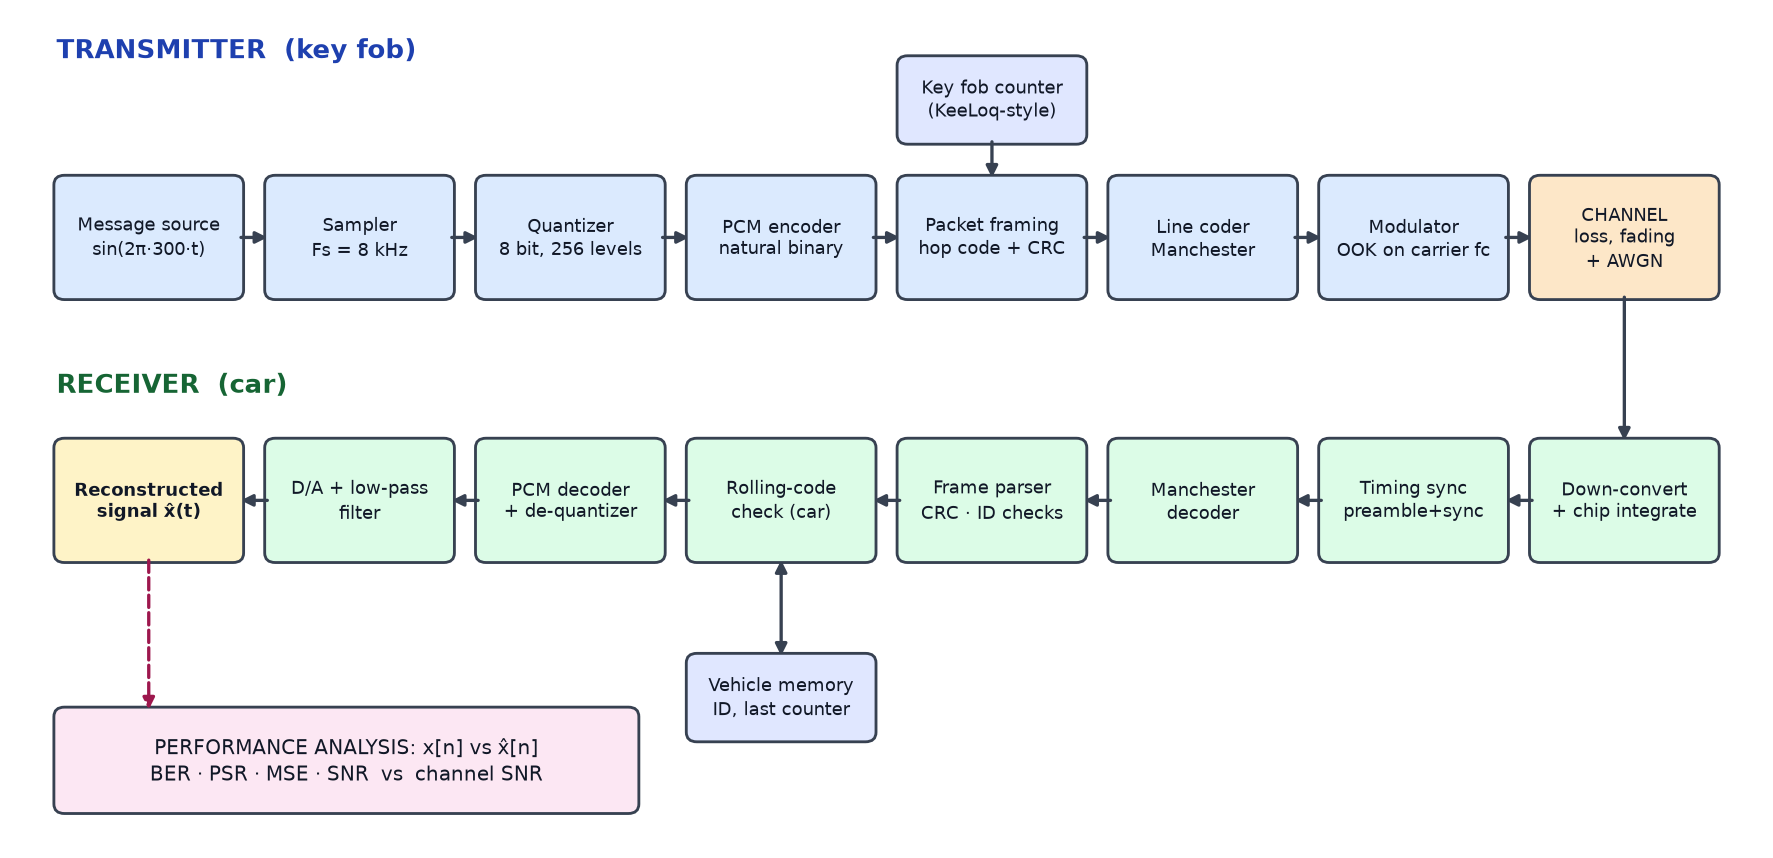
\includegraphics[width=\linewidth]{01_block_diagram.png}
\caption{Block diagram of the complete simulated system (top: key fob, bottom: car).}\label{fig:block}\end{figure}

\begin{table}[H]\centering\small
\caption{System parameters (all in \texttt{functions/config.py}).}\label{tab:params}
\begin{tabular}{@{}lll@{}}\toprule
Parameter & Value & Comment\\\midrule
Message & 300 Hz sine, amplitude 1, 50 ms & guideline values\\
Sampling rate $F_s$ & 8 kHz (400 samples) & 15 message periods\\
PCM & 8 bit $\Rightarrow$ 3200 payload bits & $\Delta=@DELTA@$\\
Packet & 3320 bits (Fig.~\ref{fig:packet}) & @AIRTIME@ ms on air\\
Bit rate $R_b$ & 9.6 kbit/s & typical RKE value\\
Line code & Manchester, 19.2 kchip/s & 16 samples per chip\\
Modulation & OOK, scaled carrier $f_c=38.4$ kHz & real fobs: 315/433.92 MHz\\
Simulation rate & $f_{s,rf}=307.2$ kHz & 8 samples per carrier cycle\\
RF bandwidth $B$ & $4R_b=38.4$ kHz (null-to-null) & Manchester $\times$ OOK\\
Channel & path loss, block fading, AWGN & Sec.~\ref{sec:range}\\
Monte Carlo & @N_SWEEP@ packets per SNR point (@BITS_PT@ Mbit) & seed 2026\\\bottomrule
\end{tabular}
\end{table}

\paragraph{Why a scaled carrier.} Simulating 433.92 MHz would need a sampling rate of several GHz. The error performance of a pass-band link depends on
$\EbNo$ and not on $f_c$ as long as the carrier is much faster than the bit rate, so we use $f_c=38.4$~kHz, an integer number of carrier cycles per chip.
The path-loss model in Sec.~\ref{sec:range} still uses the real 433.92~MHz.

%=====================================================================================
\section{The chain stage by stage}
All figures of this section come from one representative packet sent at a channel SNR of $+2$~dB (unless stated otherwise).

\subsection{Source and sampling}
The message is $x(t)=\sin(2\pi f_m t)$ with $f_m=300$~Hz, drawn on a fine 64~kHz grid to play the role of the analog signal. The ideal sampler keeps every eighth point
($F_s=8$~kHz, Nyquist frequency 4~kHz $\gg f_m$, so no aliasing and no anti-alias filter is needed).

\begin{figure}[H]\centering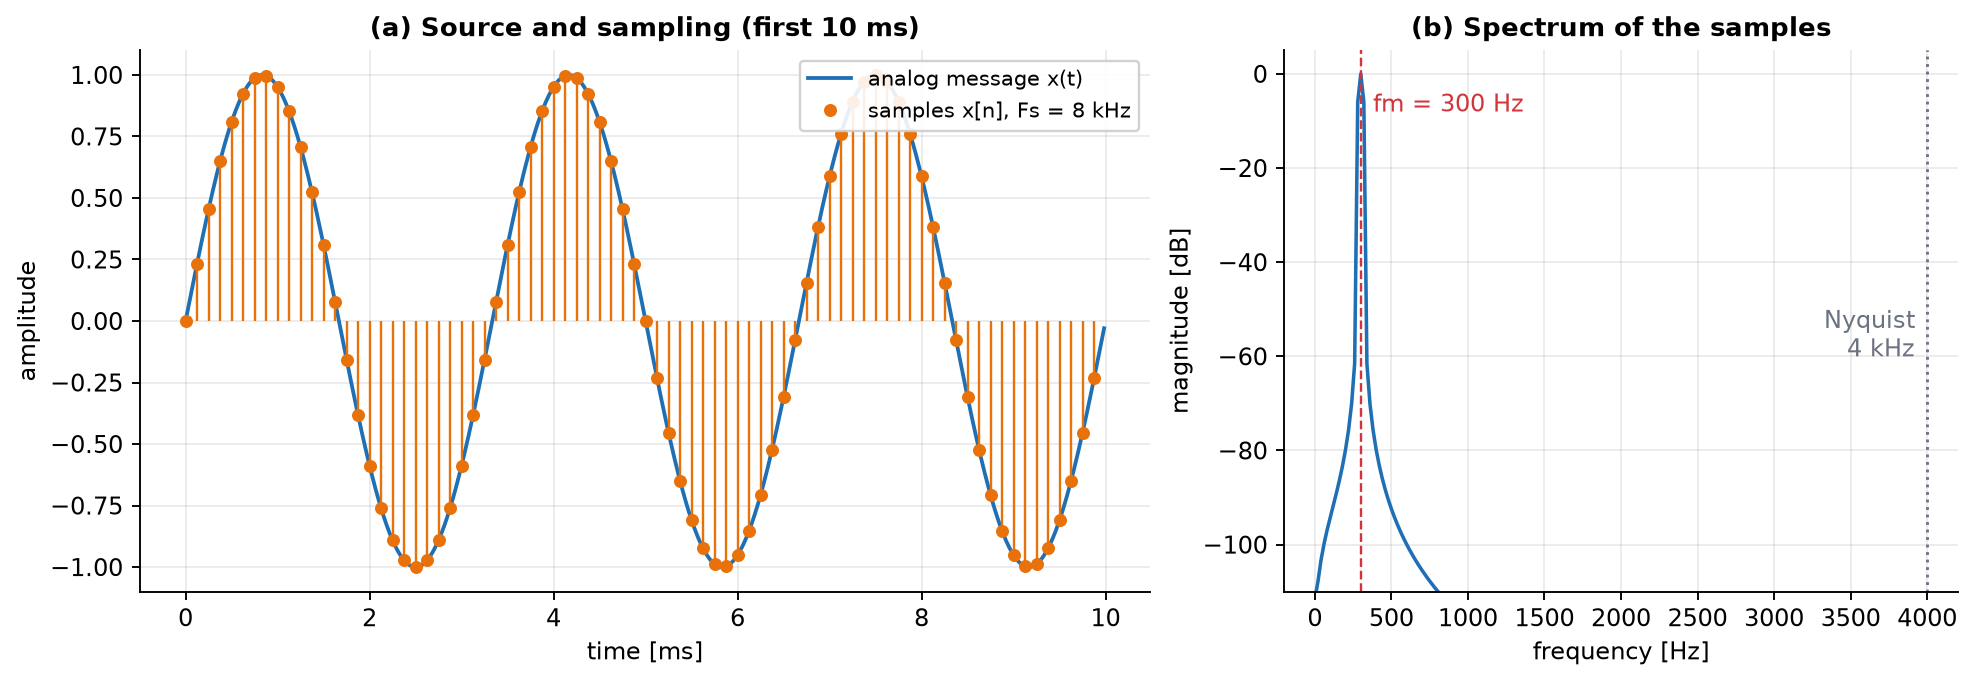
\includegraphics[width=\linewidth]{02_source_sampling.png}
\caption{(a) Analog message and its samples. (b) Spectrum of the samples: a single line at 300 Hz.}\end{figure}

\subsection{Quantization and PCM}
The uniform mid-rise quantizer has $L=2^n=256$ levels over $[-1,1]$, step $\Delta=2/256=@DELTA@$ and error $|e|\le\Delta/2$.
For a full-scale sine the theoretical signal-to-quantization-noise ratio is $\mathrm{SQNR}=6.02\,n+1.76=@SQNR_TH@$~dB. We \emph{measure} @SQNR@~dB
(MSE $=$ @MSEQ@): the 400 samples contain only 80 distinct phases (300 Hz at 8 kHz repeats every 3 periods), so the error is not perfectly uniform and
lands about 1~dB below the textbook value. This is the \textbf{quantization floor} of the whole system: no channel, however good, can push the MSE below it.

\begin{figure}[H]\centering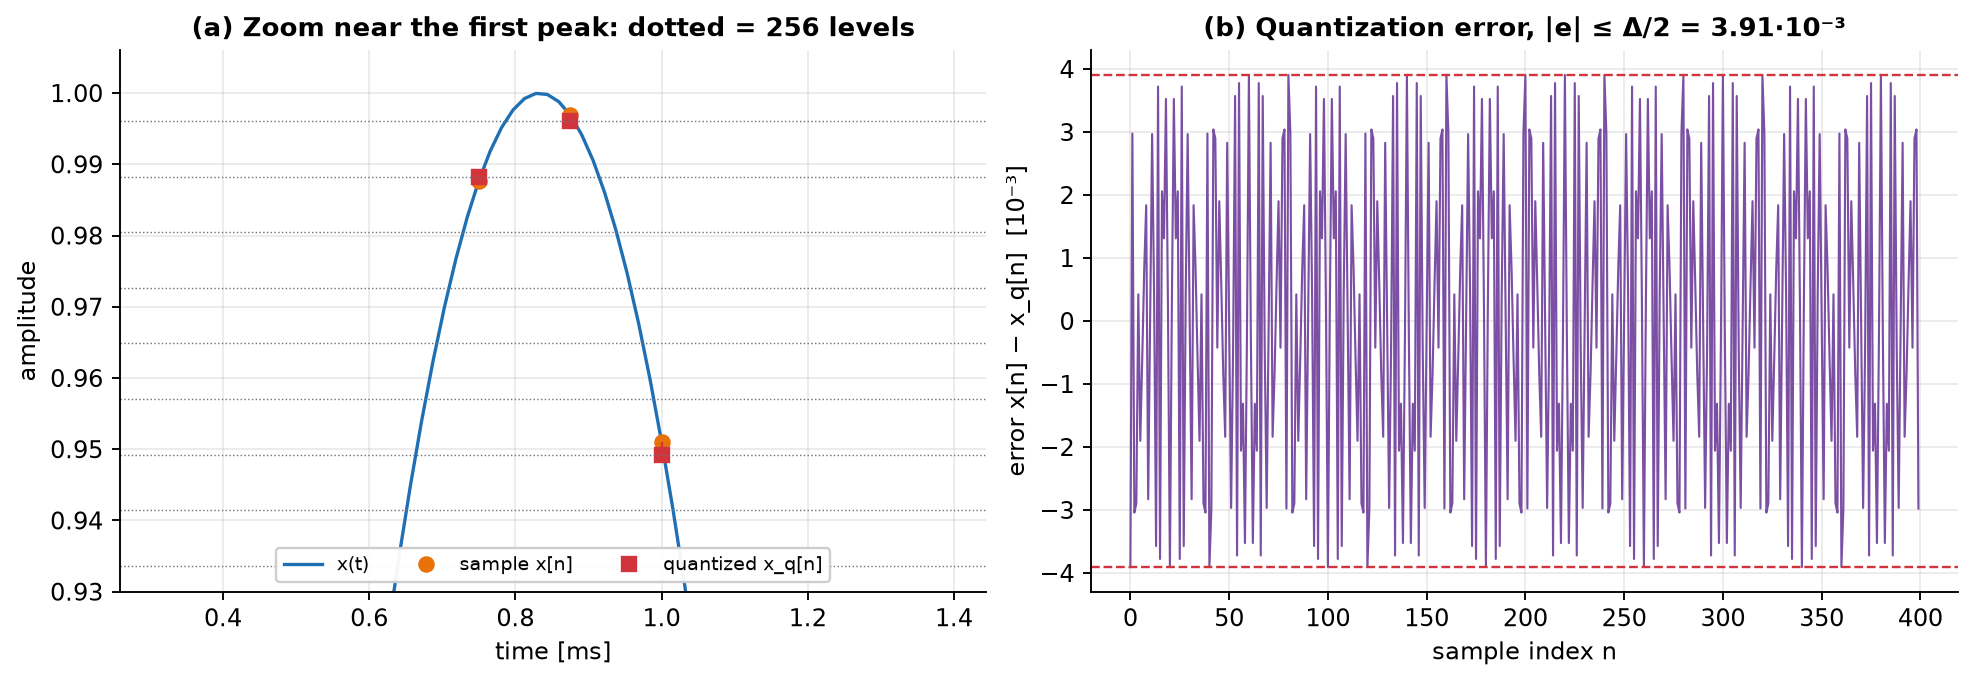
\includegraphics[width=\linewidth]{03_quantization.png}
\caption{(a) Zoom near the first peak: samples (orange) are moved to the nearest of the 256 levels (red). (b) Quantization error over all samples.}\end{figure}

Every level index is written as an 8-bit natural-binary word, MSB first (\texttt{pcm.py}); the 400 words give the 3200-bit payload.

\begin{figure}[H]\centering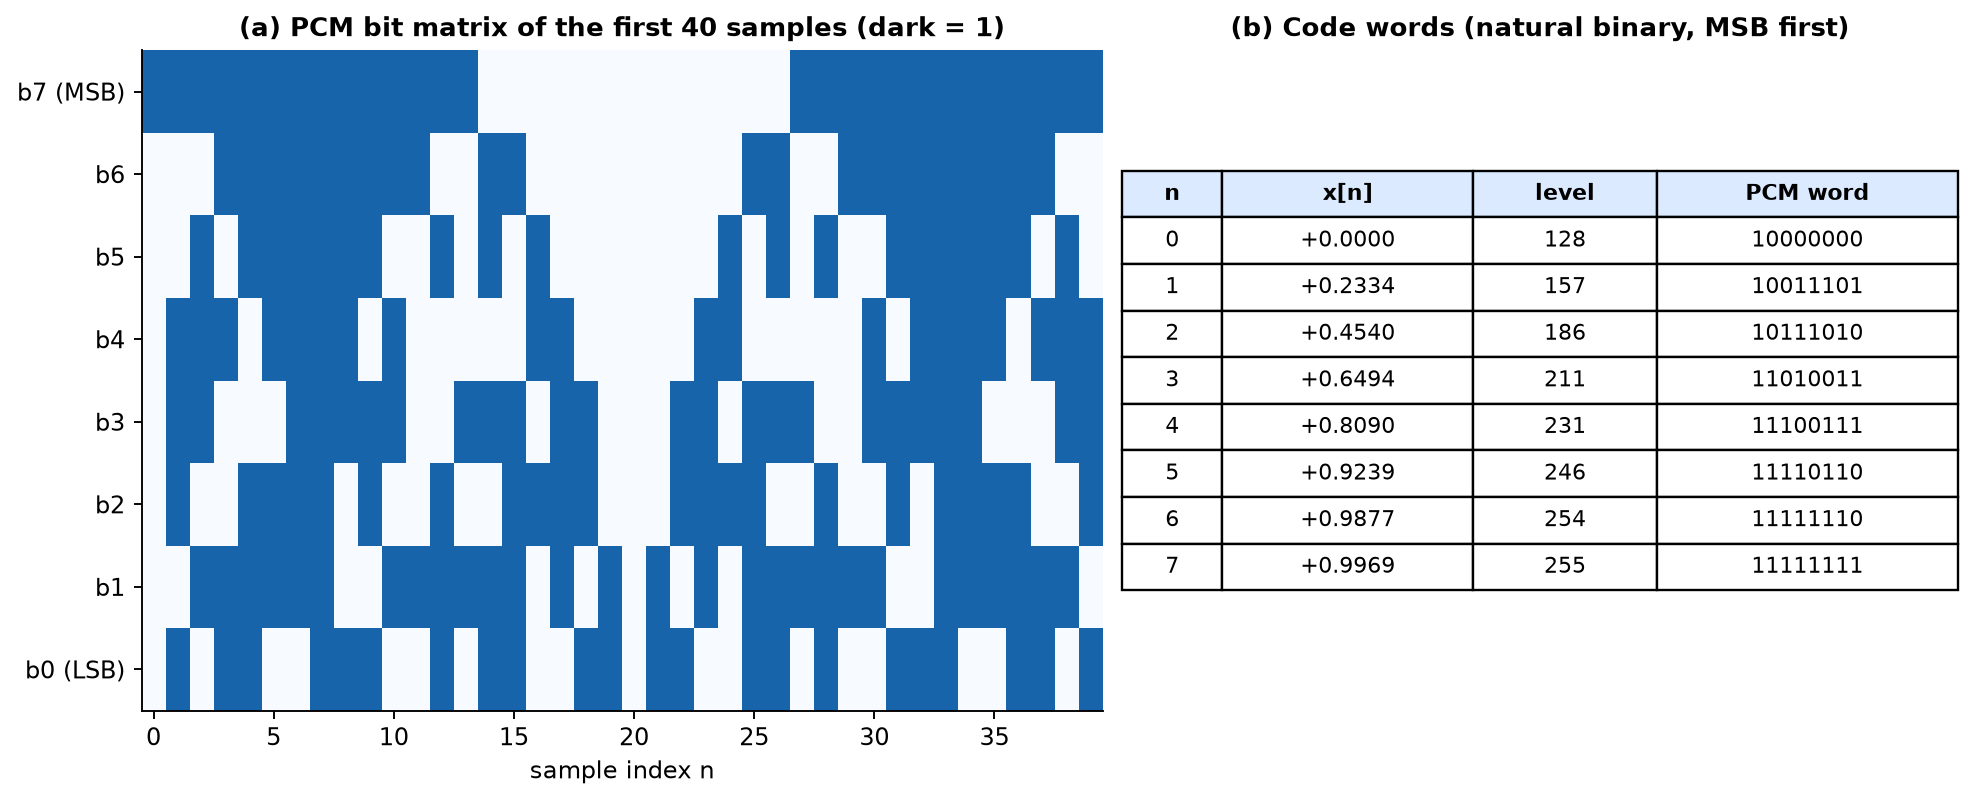
\includegraphics[width=\linewidth]{04_pcm_encoding.png}
\caption{PCM bit matrix and the first code words. The MSB (top row) toggles with the sign of the message, the LSB looks random.}\end{figure}

\subsection{Packet framing, CRC and rolling code}
The payload is wrapped in the fob frame of Fig.~\ref{fig:packet}. The 16-bit preamble ($\texttt{0xAAAA}$) is a clock/gain training pattern, the sync word ($\texttt{0x2DD4}$)
marks the start of the frame, the 32-bit device ID identifies the fob, the command byte selects lock/unlock/trunk/panic, the 32-bit \emph{hop code} is the encrypted rolling
counter (Sec.~\ref{sec:security}) and the CRC-16/CCITT ($x^{16}+x^{12}+x^5+1$, init \texttt{0xFFFF}, check value \texttt{0x29B1} for ``123456789'') protects everything from the ID to the end of the payload.

\begin{figure}[H]\centering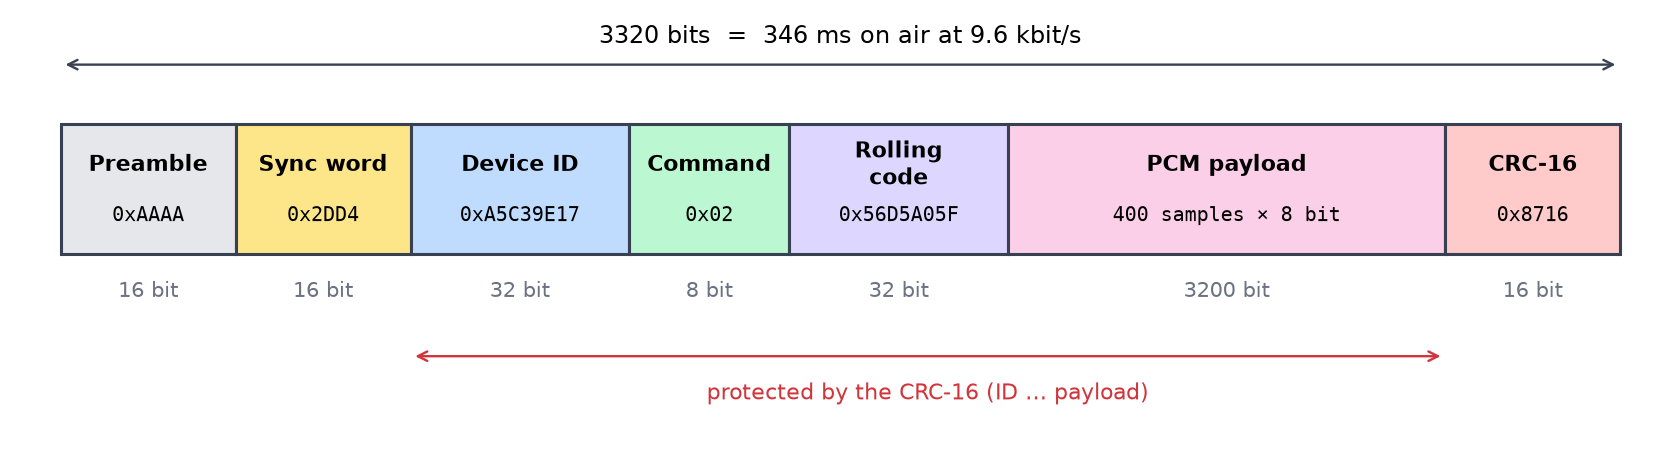
\includegraphics[width=\linewidth]{05_packet_structure.png}
\caption{Packet format (field widths not to scale). The example contents are those of the simulated packet.}\label{fig:packet}\end{figure}

\subsection{Line coding}
A \emph{chip} is one line-code symbol. NRZ-L sends one chip per bit; long runs of equal bits give no transitions, a DC component and no clock information.
Manchester sends two chips per bit, $1\to(1,0)$ and $0\to(0,1)$, which guarantees a transition in every bit (self-clocking), a 50\,\% duty cycle and --- crucial for OOK ---
a decision that compares the two halves of a bit and therefore needs \emph{no threshold}, so it keeps working when path loss changes the received amplitude.
The price is twice the bandwidth.

\begin{figure}[H]\centering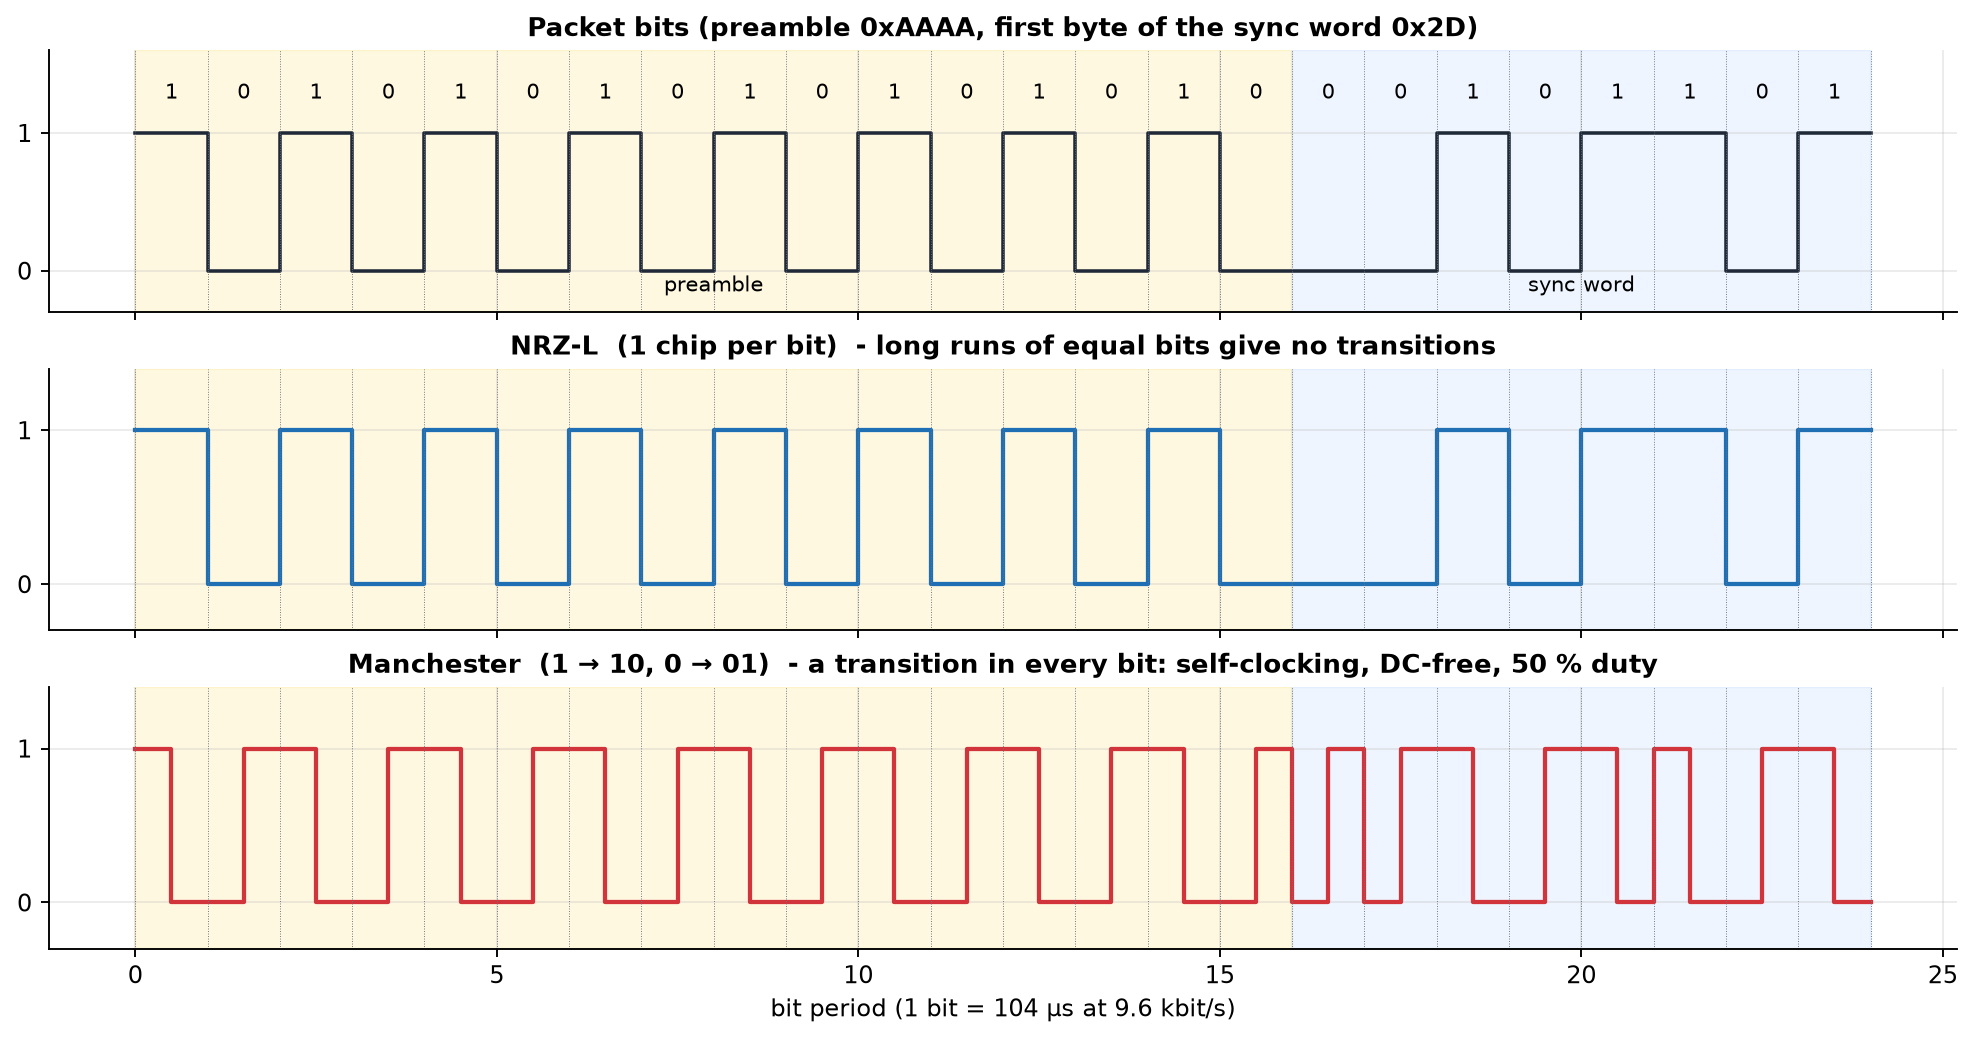
\includegraphics[width=\linewidth]{06_line_coding.png}
\caption{Packet bits, NRZ-L and Manchester waveforms for the preamble and the first byte of the sync word.}\end{figure}

\subsection{Digital modulation: OOK}
With chip $c(t)\in\{0,1\}$ the transmitted signal is $s(t)=A\,c(t)\cos(2\pi f_c t)$. Because exactly one of the two chips of every Manchester bit is ``on'', the average power is
$P=A^2/4$ and the average energy per bit is $E_b=A^2T_b/4$. The spectrum (Fig.~\ref{fig:ook}c) shows a carrier line, the Manchester null around it and nulls at $f_c\pm 2R_b$: the null-to-null
bandwidth is $B=4R_b=38.4$~kHz.

\begin{figure}[H]\centering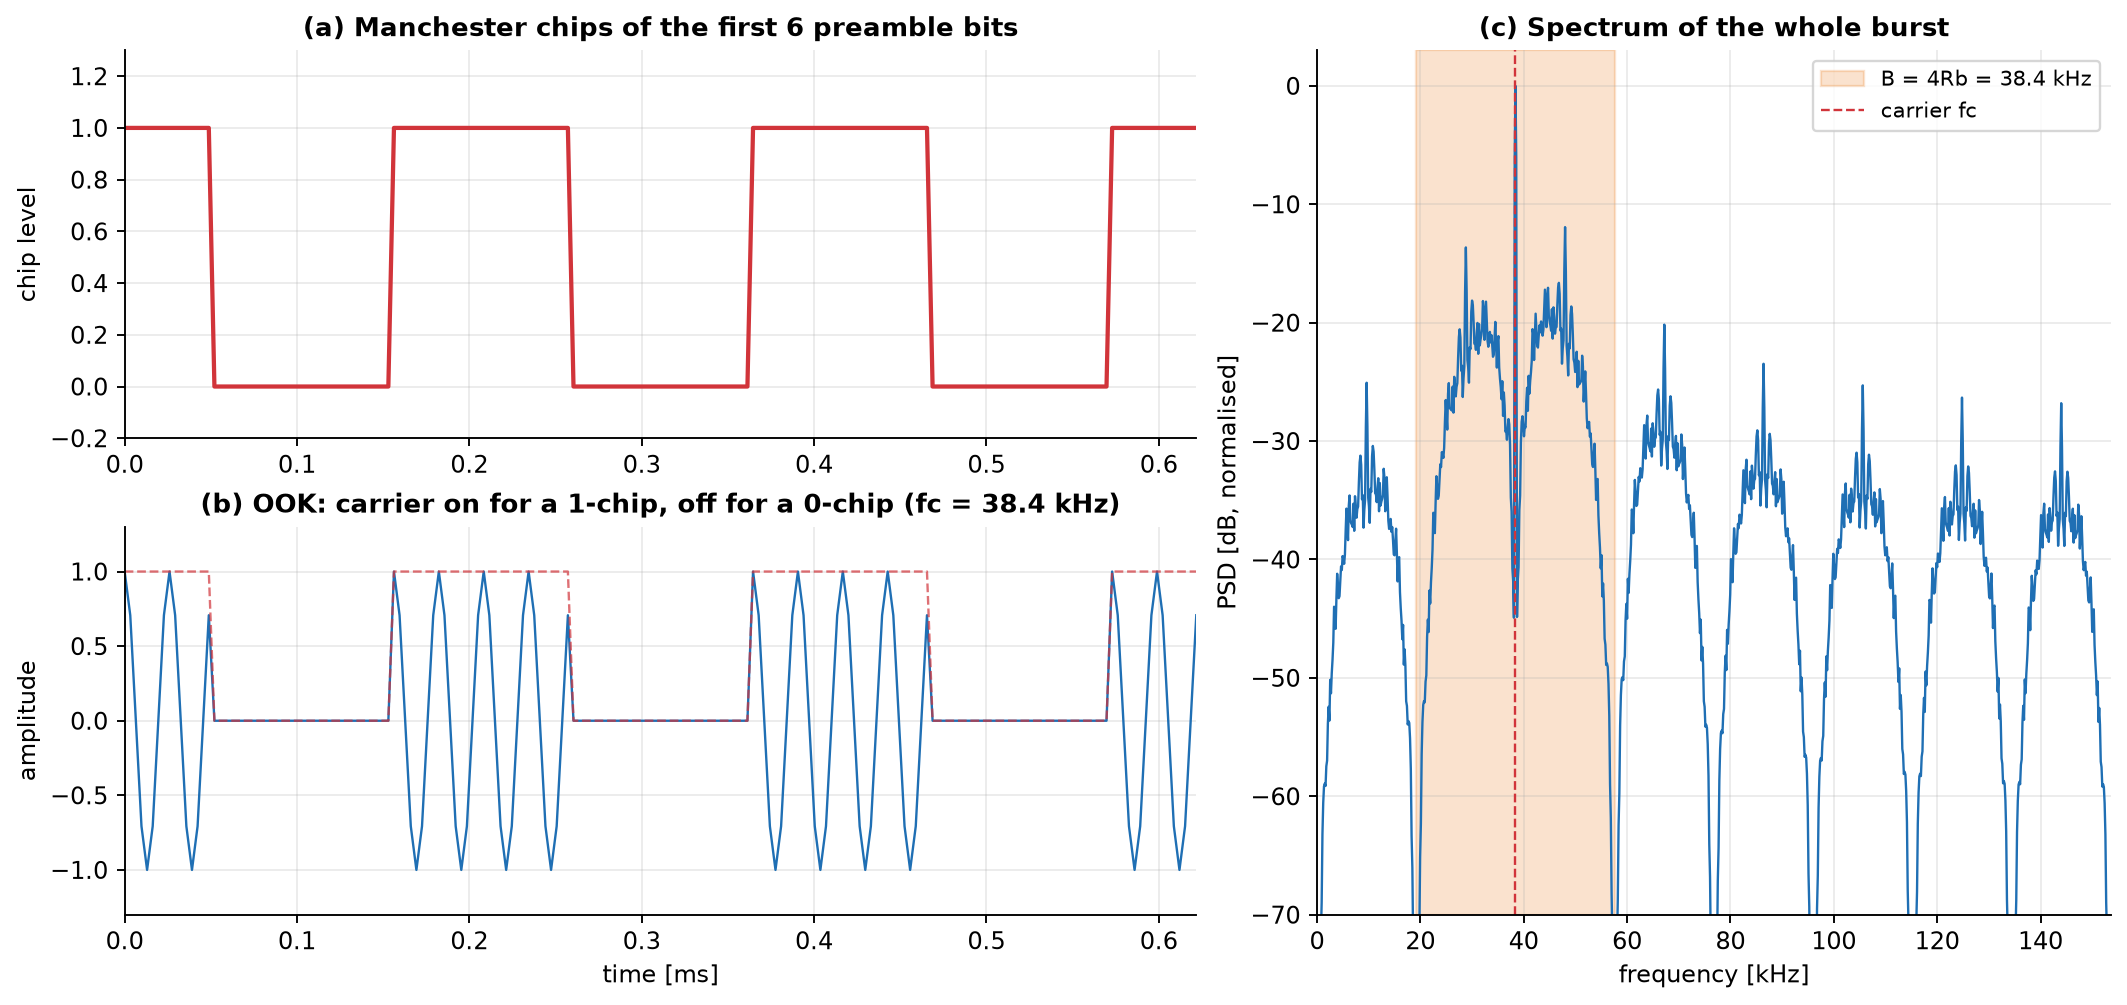
\includegraphics[width=\linewidth]{07_ook_modulation.png}
\caption{(a) Chips of the first six preamble bits, (b) the OOK burst, (c) power spectral density of the whole burst.}\label{fig:ook}\end{figure}

\subsection{Channel}
The signal is placed at a random start time in an idle record (the receiver does not know when the fob transmits), multiplied by a complex flat-fading gain $h$
(for the AWGN experiments $|h|=1$ with a random carrier phase, which the receiver does not know) and white Gaussian noise is added. We follow MATLAB's \texttt{awgn(tx,SNR,'measured')}:
\begin{equation}
\mathrm{SNR}=\frac{P_{\text{burst}}}{\sigma^2},\qquad N_0=\frac{2\sigma^2}{f_{s,rf}},\qquad
\frac{E_b}{N_0}=\mathrm{SNR}\cdot\frac{f_{s,rf}}{2R_b}\;\;\Rightarrow\;\; \frac{E_b}{N_0}\,[\text{dB}]=\mathrm{SNR}\,[\text{dB}]+@OFF_EB@\ \text{dB}.
\end{equation}
All SNR values in this report are this ``measured'' SNR unless marked \emph{in-band}. The noise of the simulation occupies $0\ldots f_{s,rf}/2=153.6$~kHz; the same noise power measured only inside the signal bandwidth $B$ is 6.02~dB \emph{higher in SNR}
(in-band SNR $=$ SNR $+6.02$~dB). The in-band SNR is the one that belongs in Shannon's formula.

\begin{figure}[H]\centering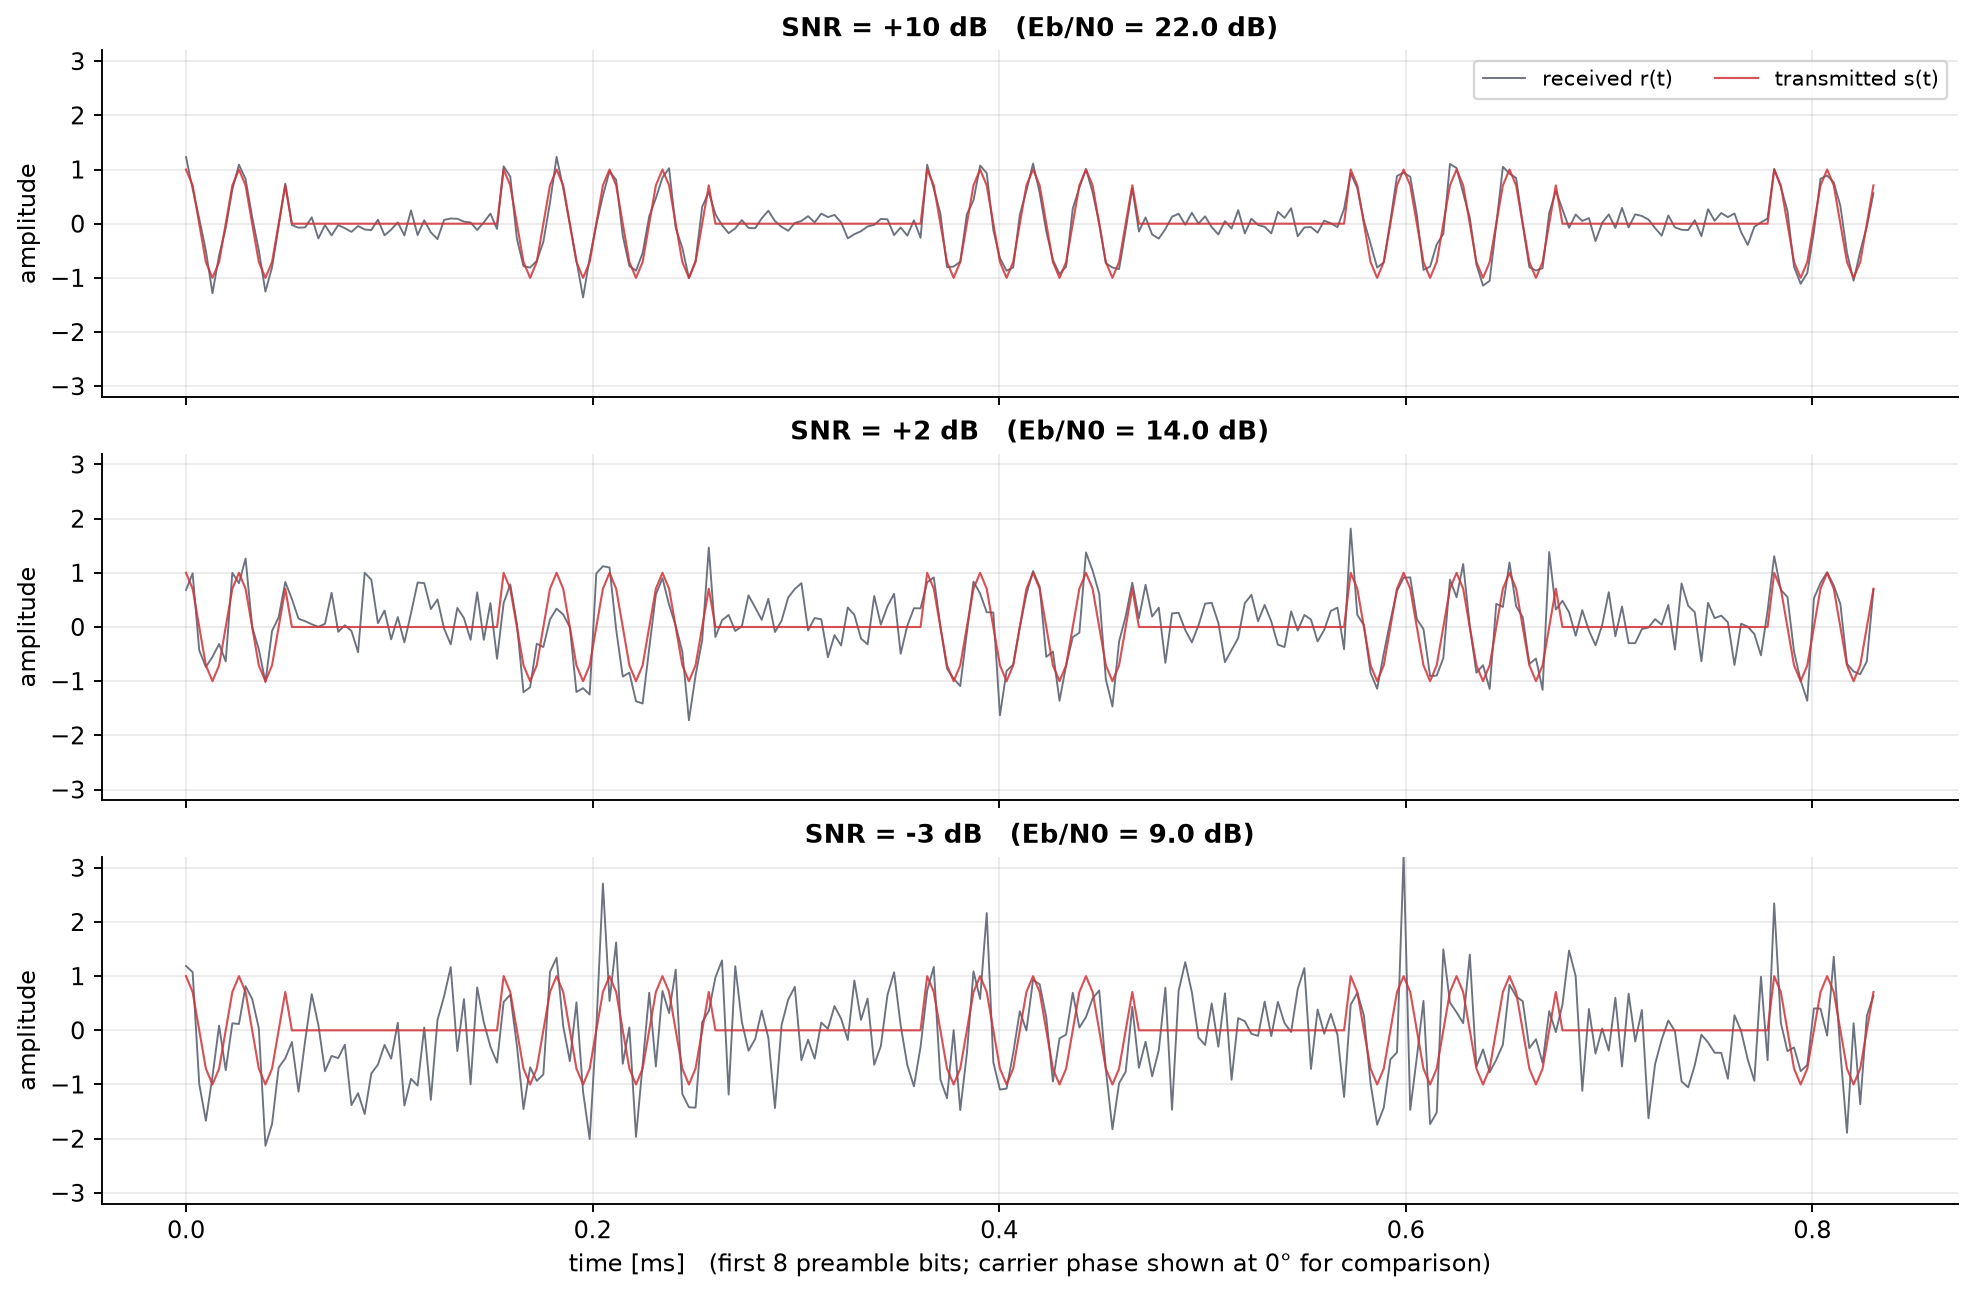
\includegraphics[width=\linewidth]{08_channel_received.png}
\caption{Transmitted (red) and received (gray) signal for three SNRs. For this plot the carrier phase is set to $0^\circ$ so that the two can be compared.}\end{figure}

\subsection{Demodulation, synchronisation and decoding}
\paragraph{Front end.} The record is mixed with $e^{-j2\pi f_c t}$ and passed through a sliding integrate-and-dump over one chip: $y[n]=\sum_{k=0}^{15} r[n+k]e^{-j\omega(n+k)}$. Because 16 samples span an integer number of carrier cycles, the double-frequency term cancels exactly and
$E[n]=|y[n]|^2$ is the energy of the chip starting at sample $n$, \emph{independent of the carrier phase} (non-coherent detection, as in real fobs).

\paragraph{Timing recovery.} The receiver does not know where the burst starts. It correlates $E[n]$ with the known $\pm1$ pattern of preamble+sync (zero mean, so the noise floor cancels) and takes the maximum over all candidate start samples (Fig.~\ref{fig:demod}b).

\paragraph{Decision.} For every bit the energies $E_1,E_2$ of the two chips are compared: bit $=1$ if $E_1>E_2$ (Fig.~\ref{fig:demod}c,d). The bits go to the frame parser which checks the sync word (up to 2 errors tolerated), the CRC-16 and the device ID, and then to the rolling-code check.

\begin{figure}[H]\centering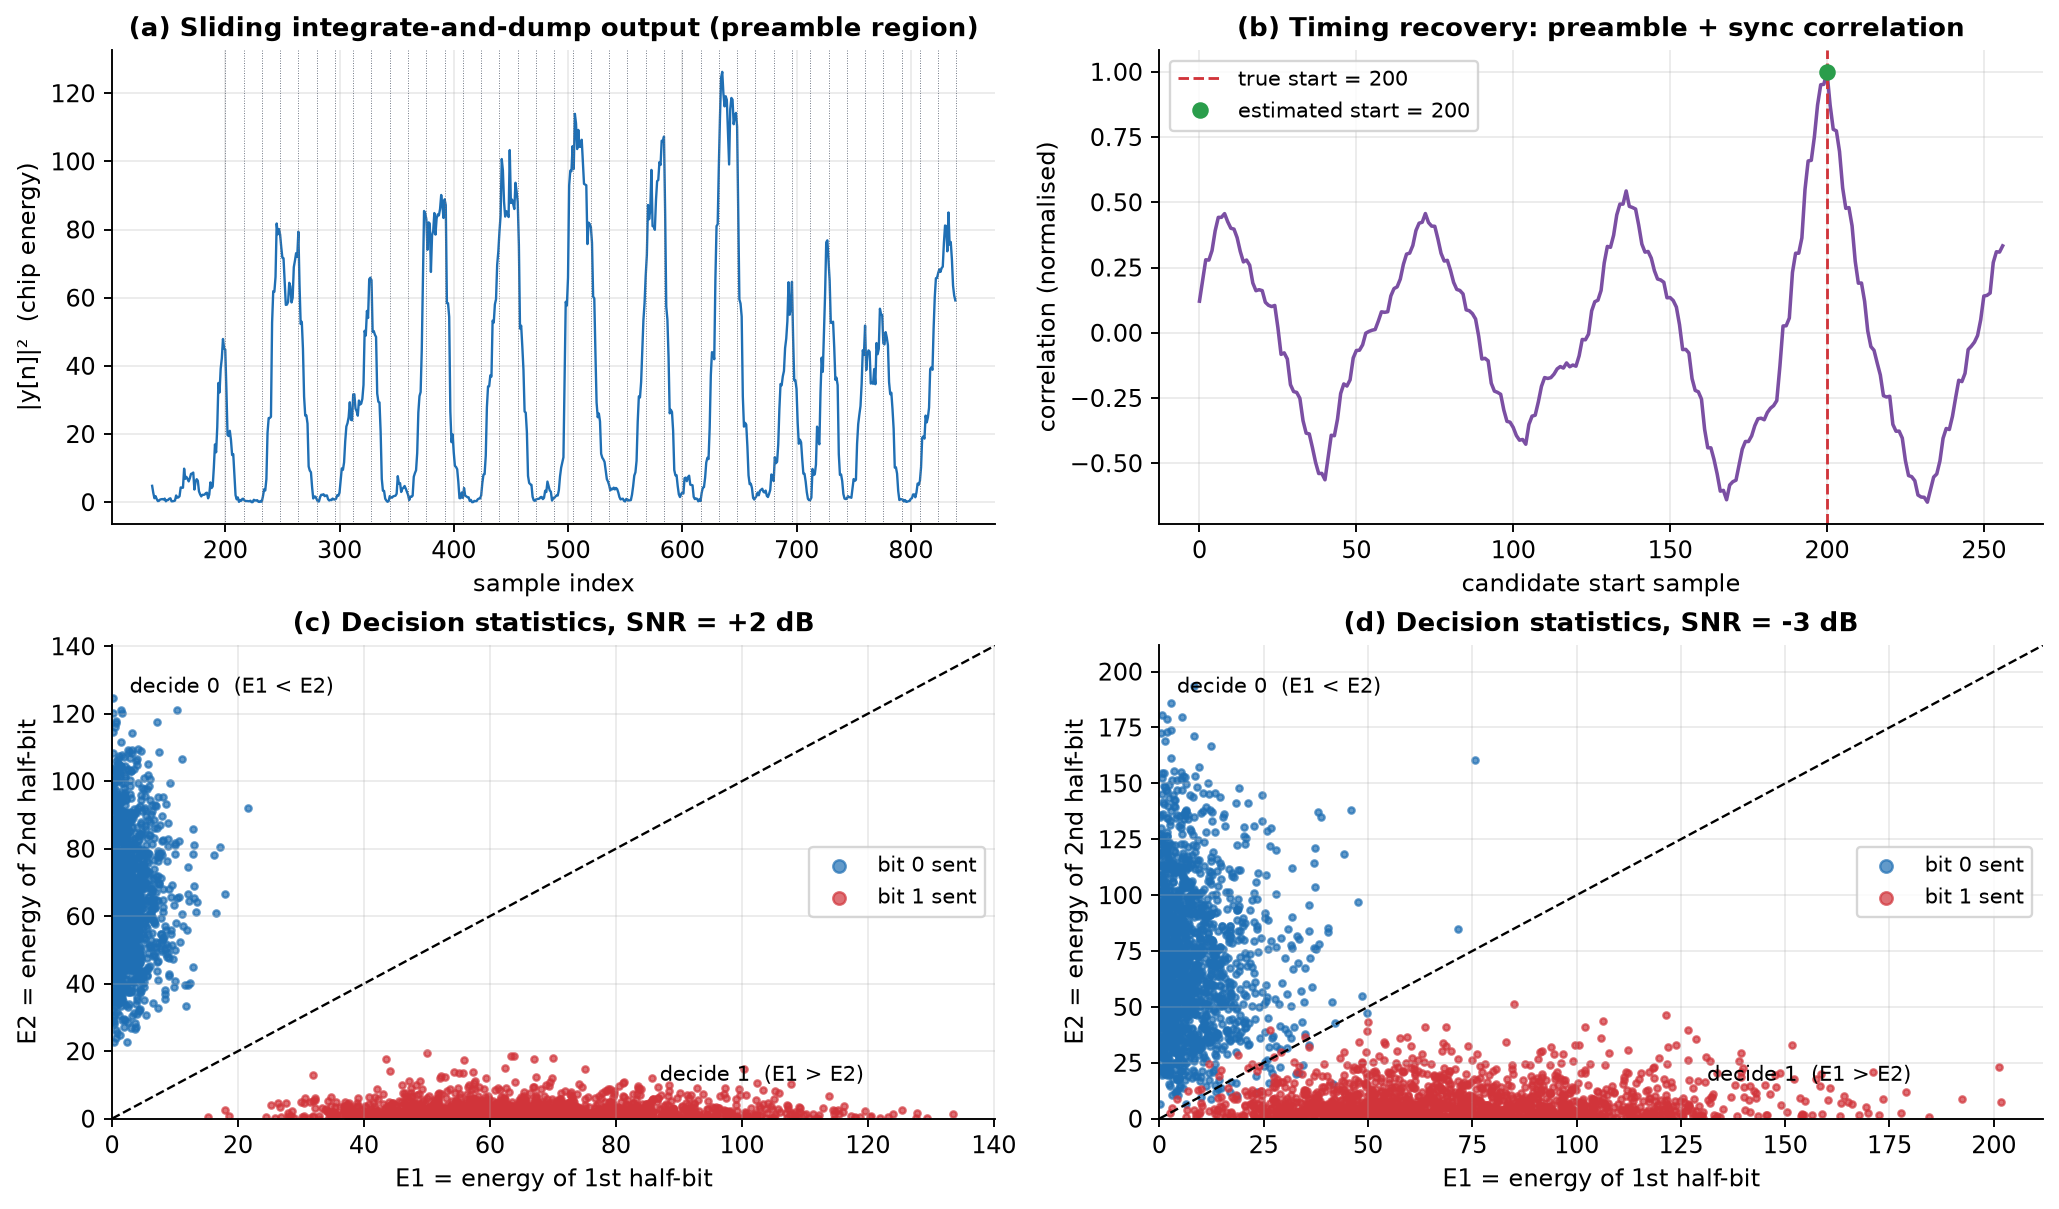
\includegraphics[width=\linewidth]{09_demodulation.png}
\caption{(a) Chip energy of the preamble. (b) Timing recovery. (c,d) Decision plane at $+2$~dB and $-3$~dB.}\label{fig:demod}\end{figure}

\begin{figure}[H]\centering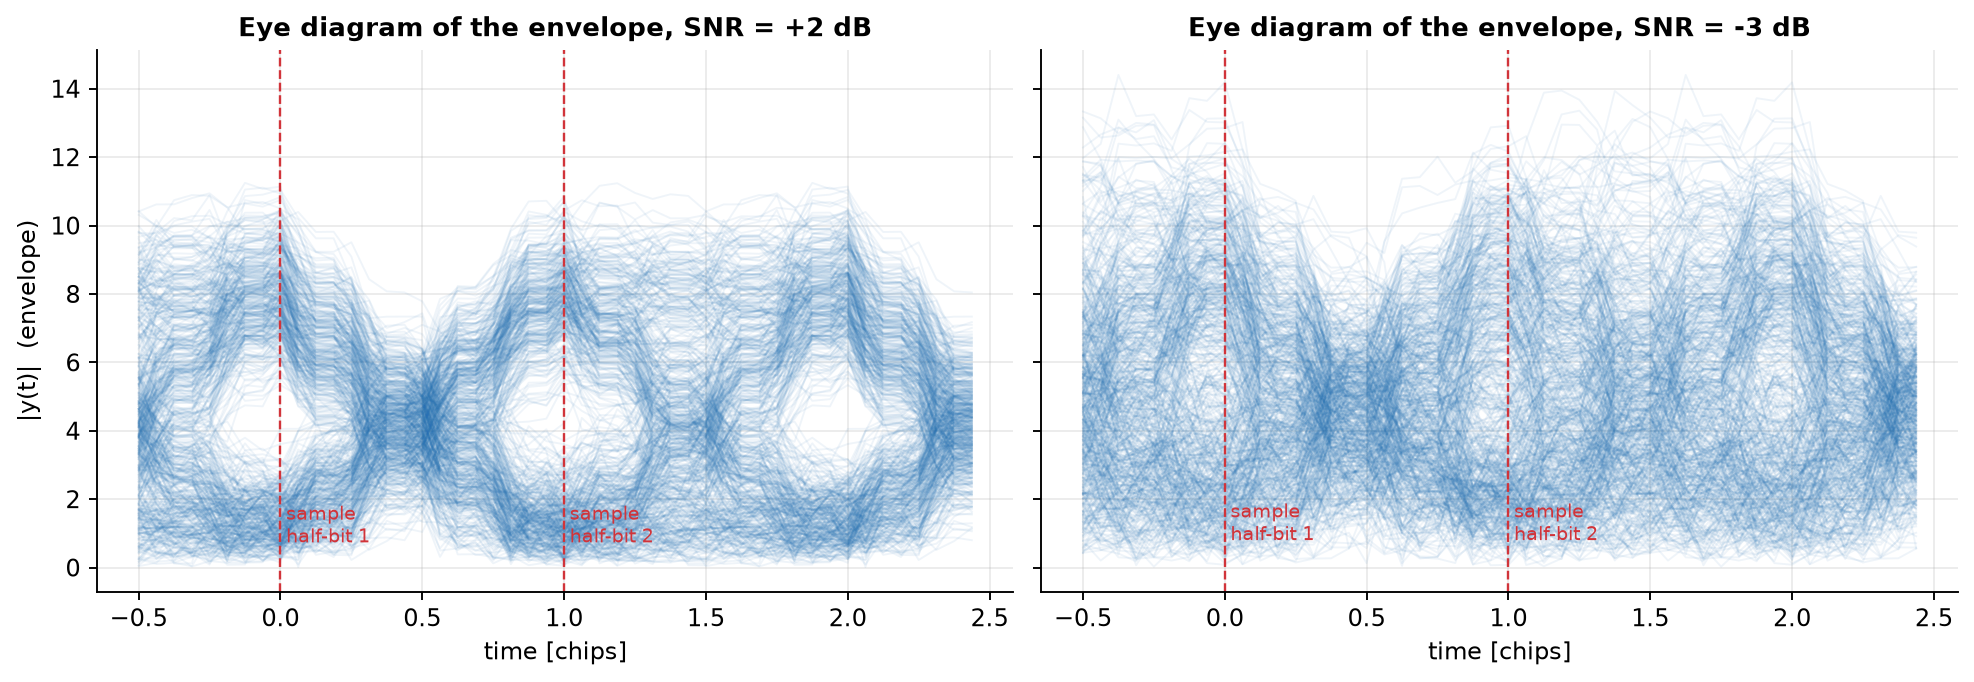
\includegraphics[width=0.95\linewidth]{10_eye_diagram.png}
\caption{Eye diagram of the received envelope; the sampling instants are the red lines. The eye closes as the SNR drops.}\end{figure}

\begin{figure}[H]\centering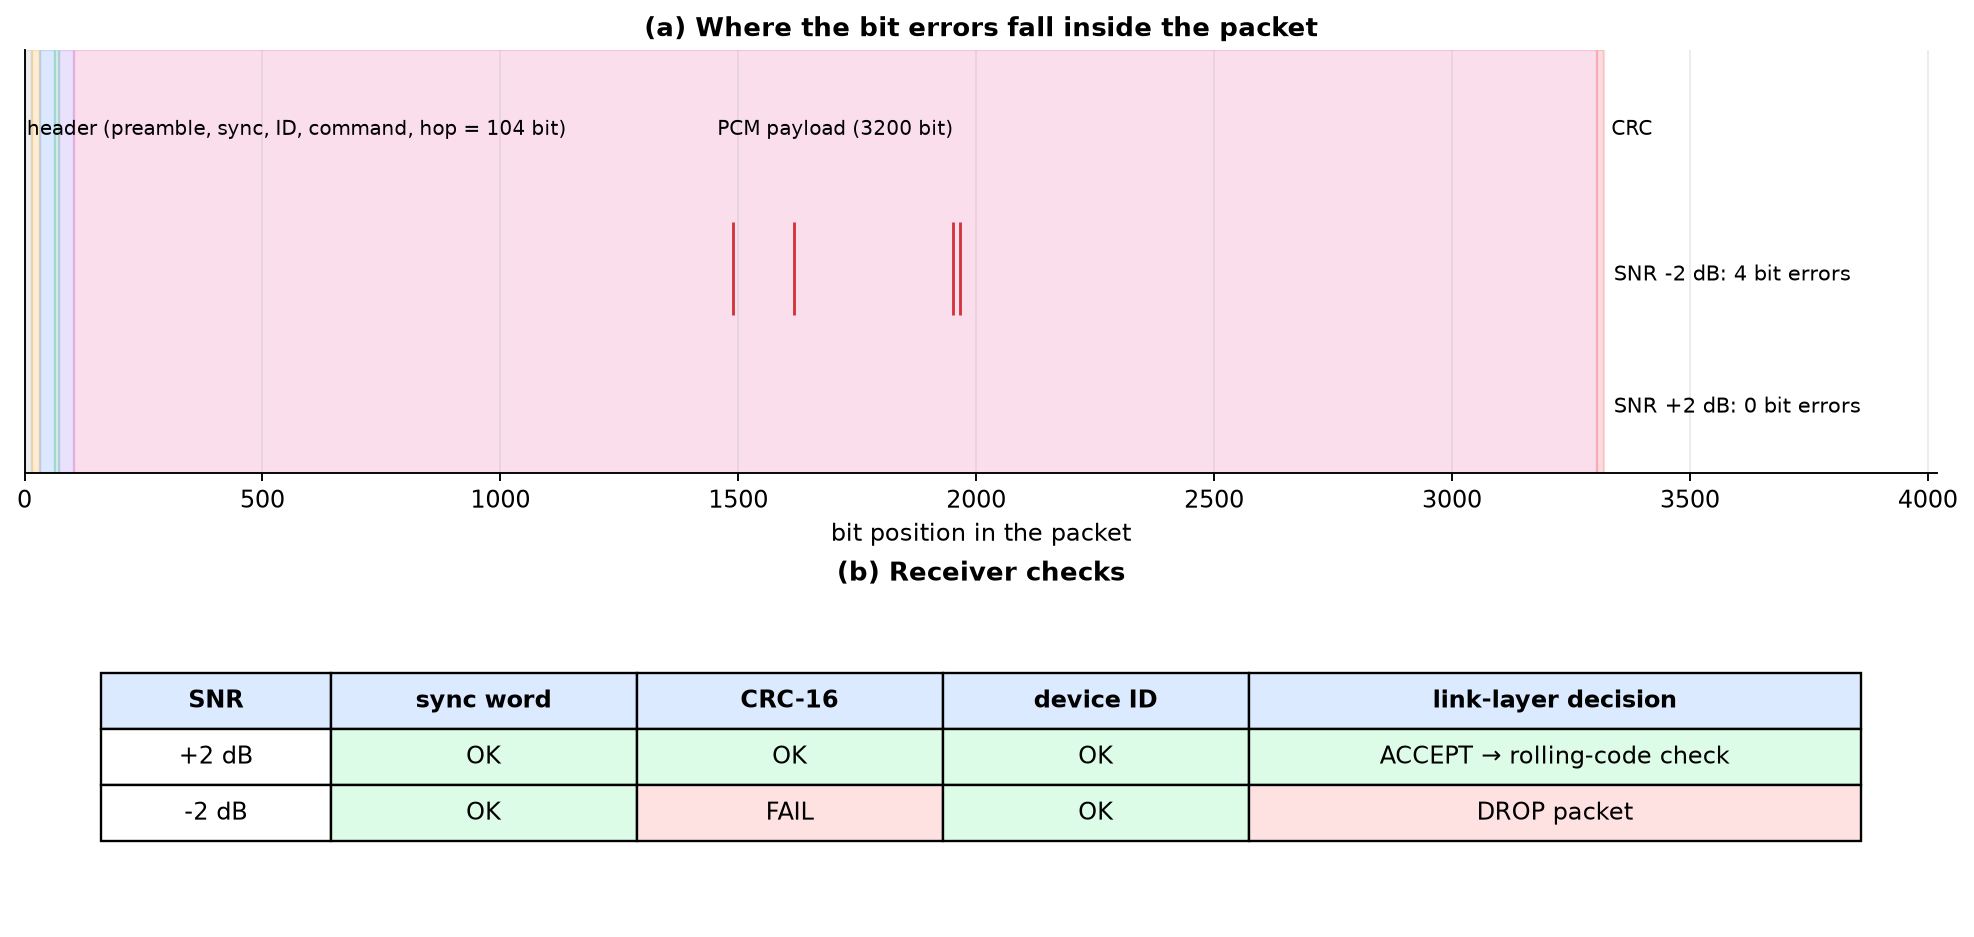
\includegraphics[width=\linewidth]{11_frame_parser.png}
\caption{Frame parser: error positions and integrity checks for a good and a corrupted packet. A few errors in the payload are enough to fail the CRC and drop the packet.}\end{figure}

\subsection{PCM decoding and reconstruction}
The payload bits are regrouped into 8-bit words, converted to the mid-point level of each quantization interval and sent through a D/A converter modelled as a zero-order hold followed by a 6th-order Butterworth low-pass at 3.4~kHz (zero-phase, half-sample hold delay compensated).
The \textbf{reconstruction MSE} is measured on the samples, $\mathrm{MSE}=\frac1N\sum_n (x[n]-\hat x[n])^2$, and the reconstruction SNR is $10\log_{10}(P_x/\mathrm{MSE})$ with $P_x=0.5$.

\begin{figure}[H]\centering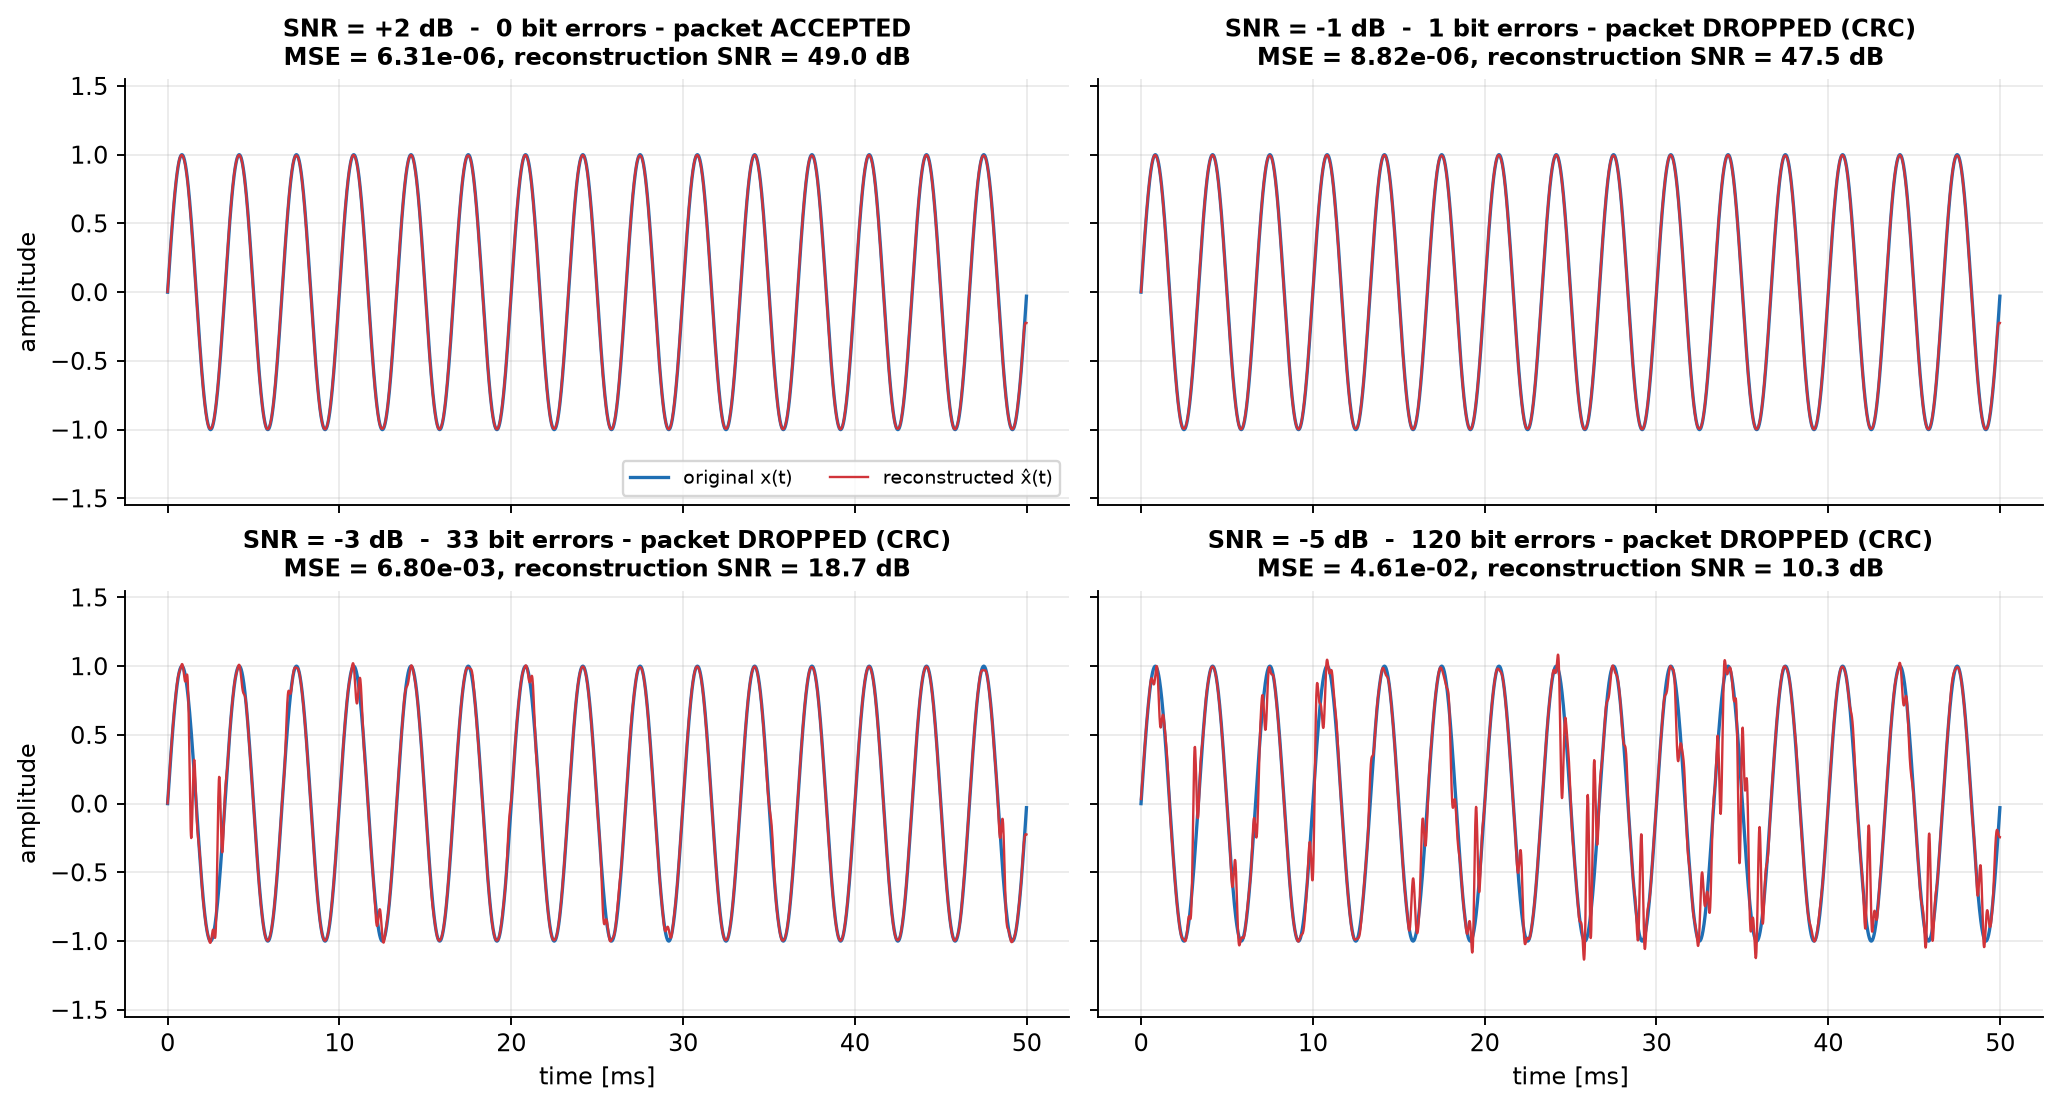
\includegraphics[width=\linewidth]{12_reconstruction.png}
\caption{Original and reconstructed message at four channel SNRs (the receiver output \emph{before} the CRC decision, i.e.\ the raw decoded payload). Single bit errors in the most significant bits appear as large spikes.}\label{fig:recon}\end{figure}

%=====================================================================================
\section{Performance analysis: channel SNR versus reconstruction quality}
For each of 19 SNR values from $-8$ to $+20$~dB we sent @N_SWEEP@ complete packets (@BITS_PT@ Mbit per point) through the whole chain with a random start time and random carrier phase, using the real (blind-timing) receiver.
Table~\ref{tab:sweep} summarises the results; all curves are in the figures that follow.

\subsection{Bit error rate}
For non-coherent detection of two orthogonal ``on-chip'' hypotheses with $E_b$ the average energy per bit, $P_b=\tfrac12\exp\!\bigl(-E_b/2N_0\bigr)$; for the textbook coherent BPSK reference $P_b=Q(\sqrt{2E_b/N_0})$.
Figure~\ref{fig:ber} shows that the simulation follows theory over four decades, which validates the modulator, channel, SNR bookkeeping, front end and detector. OOK needs about 3.8~dB more $\EbNo$ than BPSK for the same BER, the price of cheap non-coherent hardware.

\begin{figure}[H]\centering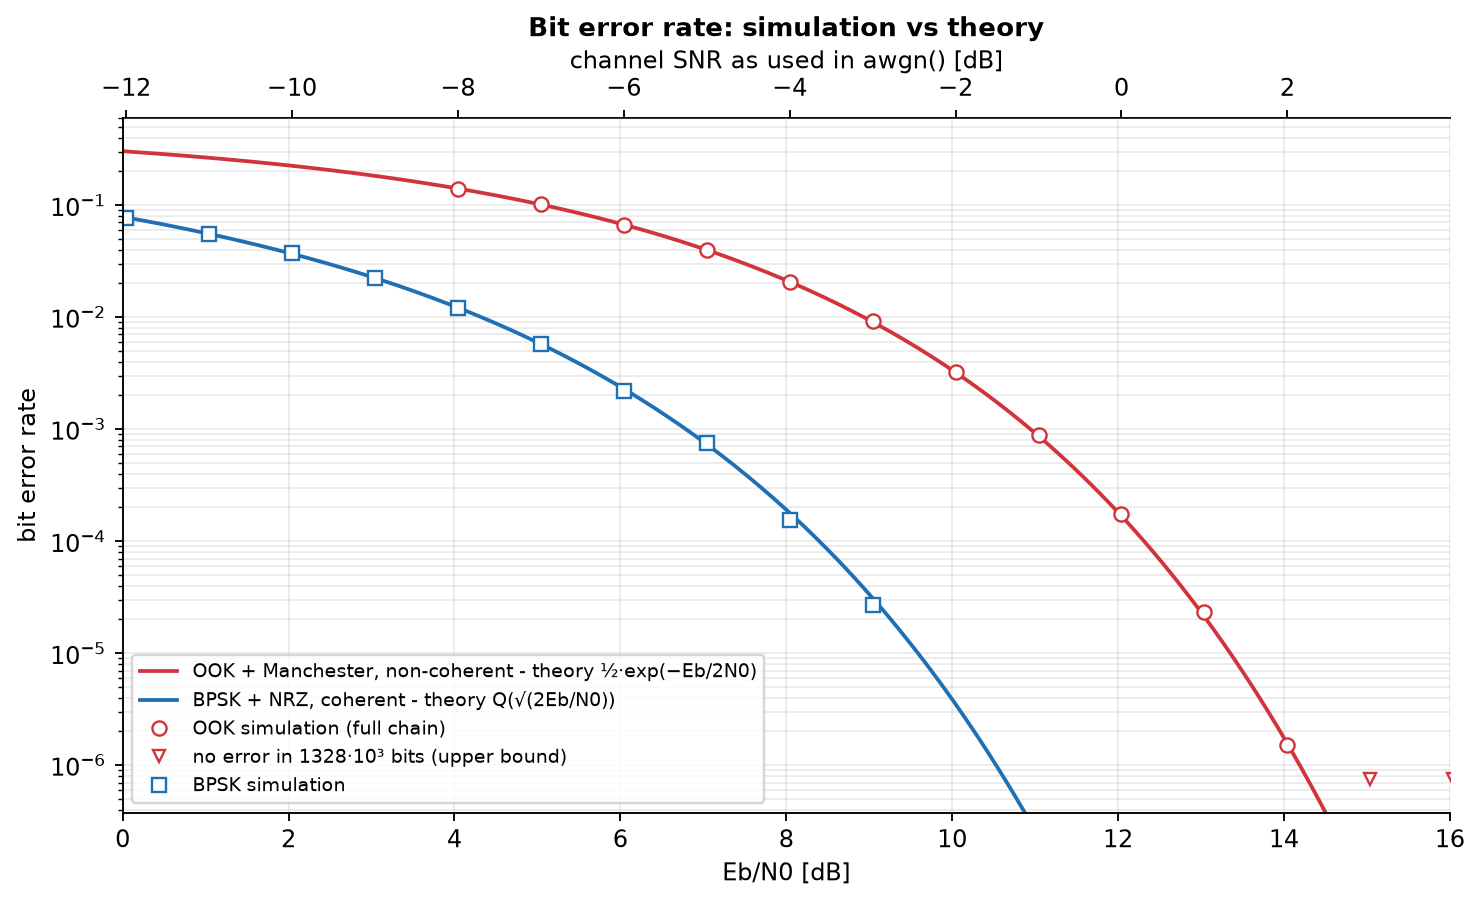
\includegraphics[width=0.82\linewidth]{13_ber_vs_snr.png}
\caption{BER versus $\EbNo$ (bottom axis) and the channel SNR used by \texttt{awgn} (top axis). Markers: Monte-Carlo, lines: theory. Down-triangles: no error seen (upper bound $1/N_{\text{bits}}$).}\label{fig:ber}\end{figure}

\subsection{MSE of the reconstructed signal}
We report three quantities. \emph{Raw}: the PCM payload is decoded whatever the receiver believes (this is the MSE asked for in the guideline). \emph{Delivered}: the car mutes the output (silence, MSE $=P_x=0.5$) whenever sync/CRC/ID fail, which is what a real receiver would do.
\emph{Theory}: the BER from theory is converted to an MSE using the actual PCM bits, assuming independent bit flips. A flip of the bit of weight $w=2^k\Delta$ shifts the decoded level by $\pm w$, so with
$e=\sum_k f_k\,\varepsilon_k w_k$ ($f_k\sim\text{Bernoulli}(p)$, $\varepsilon_k=\pm1$ from the bit value), $q=x-x_q$ and $\mathbb{E}[e]=p\sum\varepsilon_kw_k$, $\mathbb{E}[e^2]=p\sum w_k^2+p^2[(\sum\varepsilon_kw_k)^2-\sum w_k^2]$:
\begin{equation}
\mathrm{MSE}(p)=\frac1N\sum_n\Bigl(q_n^2-2q_n\mathbb{E}[e_n]+\mathbb{E}[e_n^2]\Bigr)\;\approx\;\frac{\Delta^2}{12}+p\,\Delta^2\,\frac{4^{n}-1}{3}.
\end{equation}
The second term is dominated by the MSB: one MSB error moves a sample by $128\Delta=1$, which, spread over 400 samples, raises the MSE by $2.5\times10^{-3}$ --- about 400 times the whole quantization MSE.

\begin{figure}[H]\centering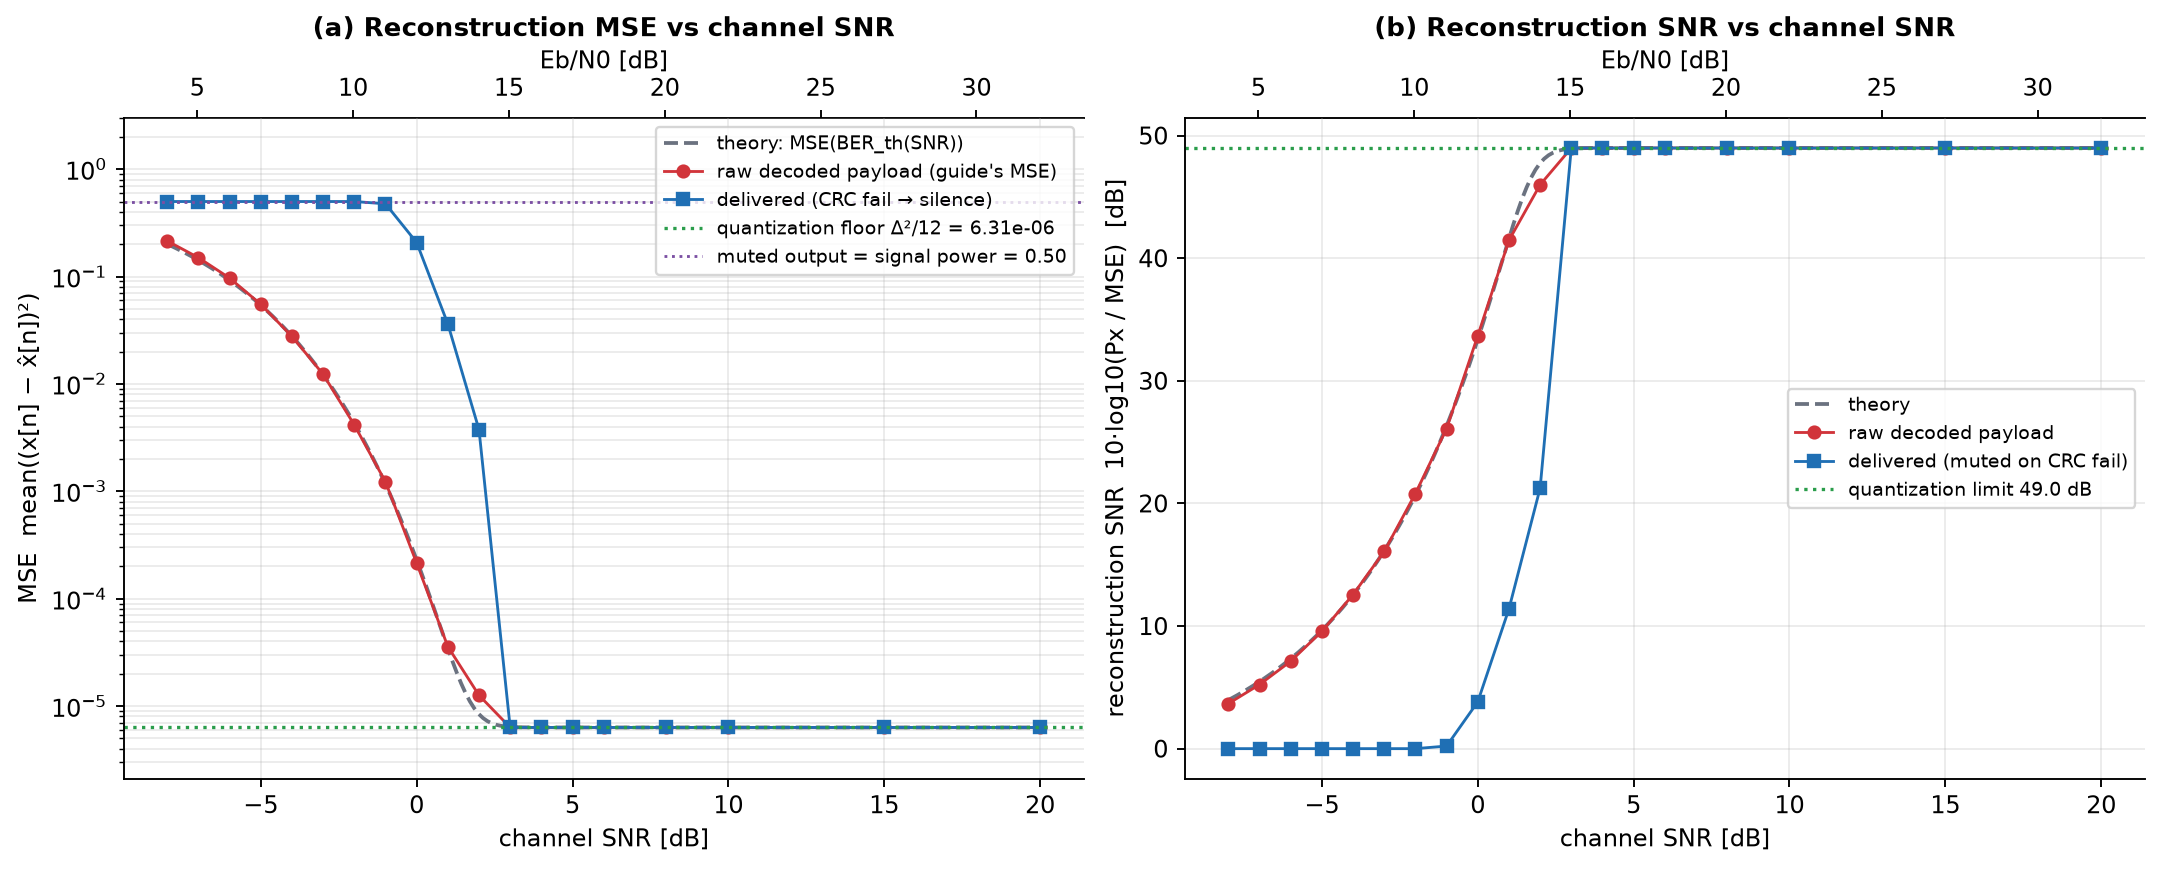
\includegraphics[width=\linewidth]{14_mse_vs_snr.png}
\caption{(a) Reconstruction MSE and (b) reconstruction SNR versus channel SNR. Markers: simulation; dashed: theory.}\label{fig:mse}\end{figure}

\begin{table}[H]\centering\small
\caption{Selected results of the SNR sweep (@N_SWEEP@ packets per row). PSR = packet success rate (sync word, CRC-16 and device ID all correct); SNR$_{\text{rec}}$ = reconstruction SNR of the raw payload.}\label{tab:sweep}
\begin{tabular}{@{}rrrrrrr@{}}\toprule
SNR [dB] & $\EbNo$ [dB] & BER & PSR & MSE (raw) & SNR$_{\text{rec}}$ [dB] & MSE (delivered)\\\midrule
@TABLE_SWEEP@
\bottomrule\end{tabular}
\end{table}

\paragraph{Reading the curves.}
\begin{itemize}[leftmargin=1.2em,itemsep=1pt]
\item \textbf{Above $\approx$ +3~dB (source-limited).} No bit errors; MSE $=$ @MSEQ@, the quantization floor, and more channel SNR cannot improve it. Only more PCM bits would.
\item \textbf{Around $-1$ to $+2$~dB (the cliff).} The BER passes from $10^{-6}$ to $10^{-3}$; the channel-induced MSE equals the quantization MSE already at $p^\ast=$ @PSTAR@, i.e.\ at $\EbNo=@EBSTAR@$~dB (SNR $=@SNRSTAR@$~dB). The reconstruction SNR falls from 49~dB at $+3$~dB to 34~dB at 0~dB and 21~dB at $-2$~dB.
\item \textbf{Below $-2$~dB (channel-limited).} BER above $3\times10^{-3}$, essentially every packet fails the CRC. Without the CRC the MSE keeps growing smoothly (the raw curve) toward $\approx0.83$, the value for random bits.
\end{itemize}
\textbf{Packet success rate.} The 90\,\% point is at SNR $=@PSR90@$~dB ($\EbNo=@PSR90_EB@$~dB), the 50\,\% point at @PSR50@~dB. In all @N_SWEEP@ packets $\times$ 19 SNR values \emph{no packet with undetected payload errors} passed the CRC.
The delivered MSE (blue) is much worse than the raw MSE around the cliff: a CRC fail discards a packet with one bad MSB, which would have given a decent (but wrong) signal. The CRC trades a bounded, known loss (silence) for protection against rare catastrophic spikes --- the right choice for a security-critical fob, the wrong one for an audio link, where one would rather conceal the error.

\begin{figure}[H]\centering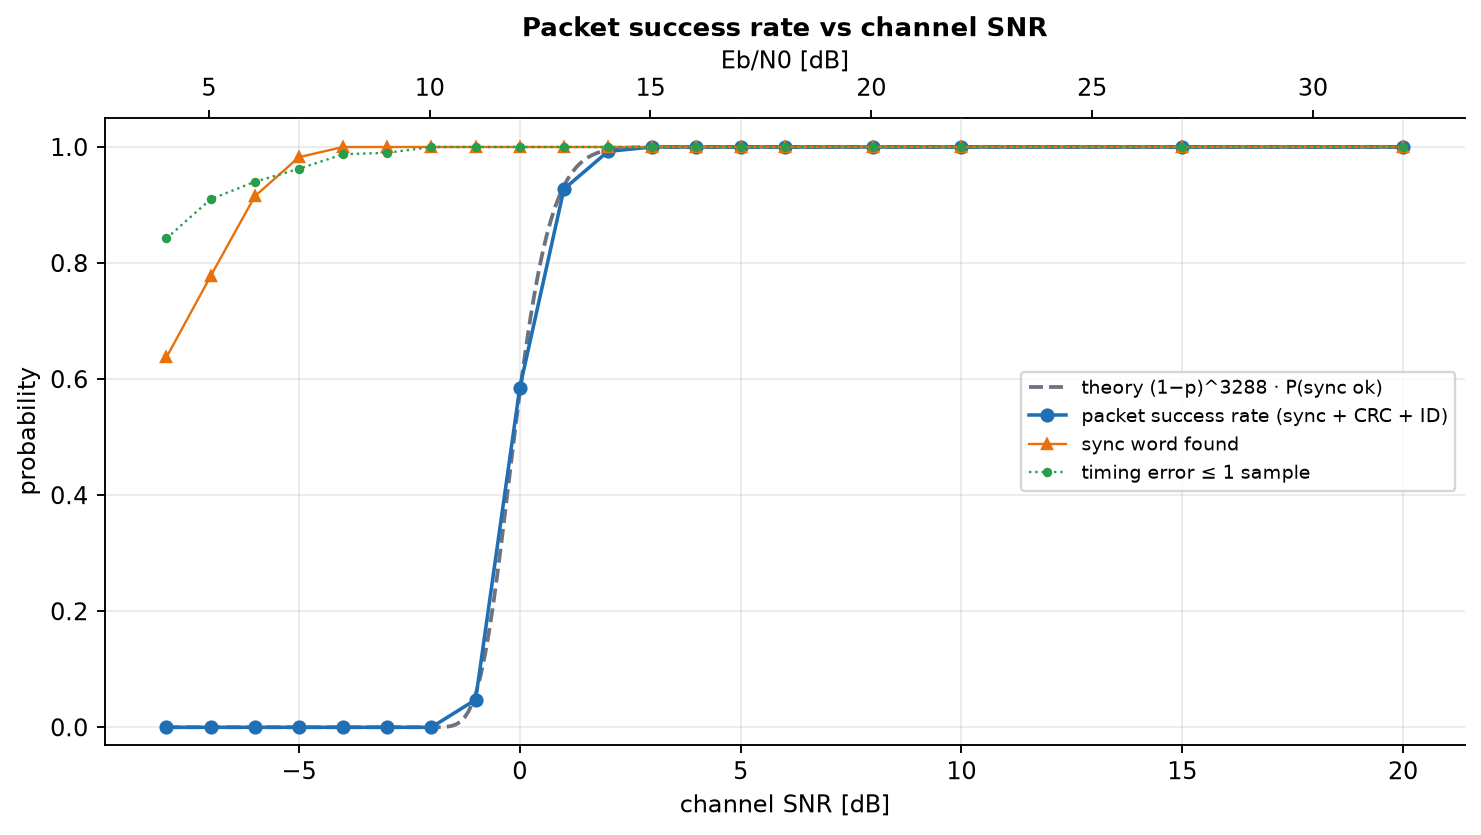
\includegraphics[width=0.82\linewidth]{15_psr_vs_snr.png}
\caption{Packet success rate versus SNR; dashed: theory $(1-p)^{3288}\cdot P(\text{sync ok})$.}\end{figure}

%=====================================================================================
\section{Link to Shannon's channel-capacity theorem}\label{sec:shannon}
Shannon's theorem states that reliable communication at rate $R$ over a channel of bandwidth $B$ and signal-to-noise ratio $S/N$ is possible \emph{if and only if} $R\le C=B\log_2(1+S/N)$. We use the in-band SNR and $B=4R_b=38.4$~kHz. Equivalently, at spectral efficiency $\eta=R_b/B$ one needs $\EbNo\ge(2^\eta-1)/\eta$, which tends to $-1.59$~dB for $\eta\to0$.

\begin{figure}[H]\centering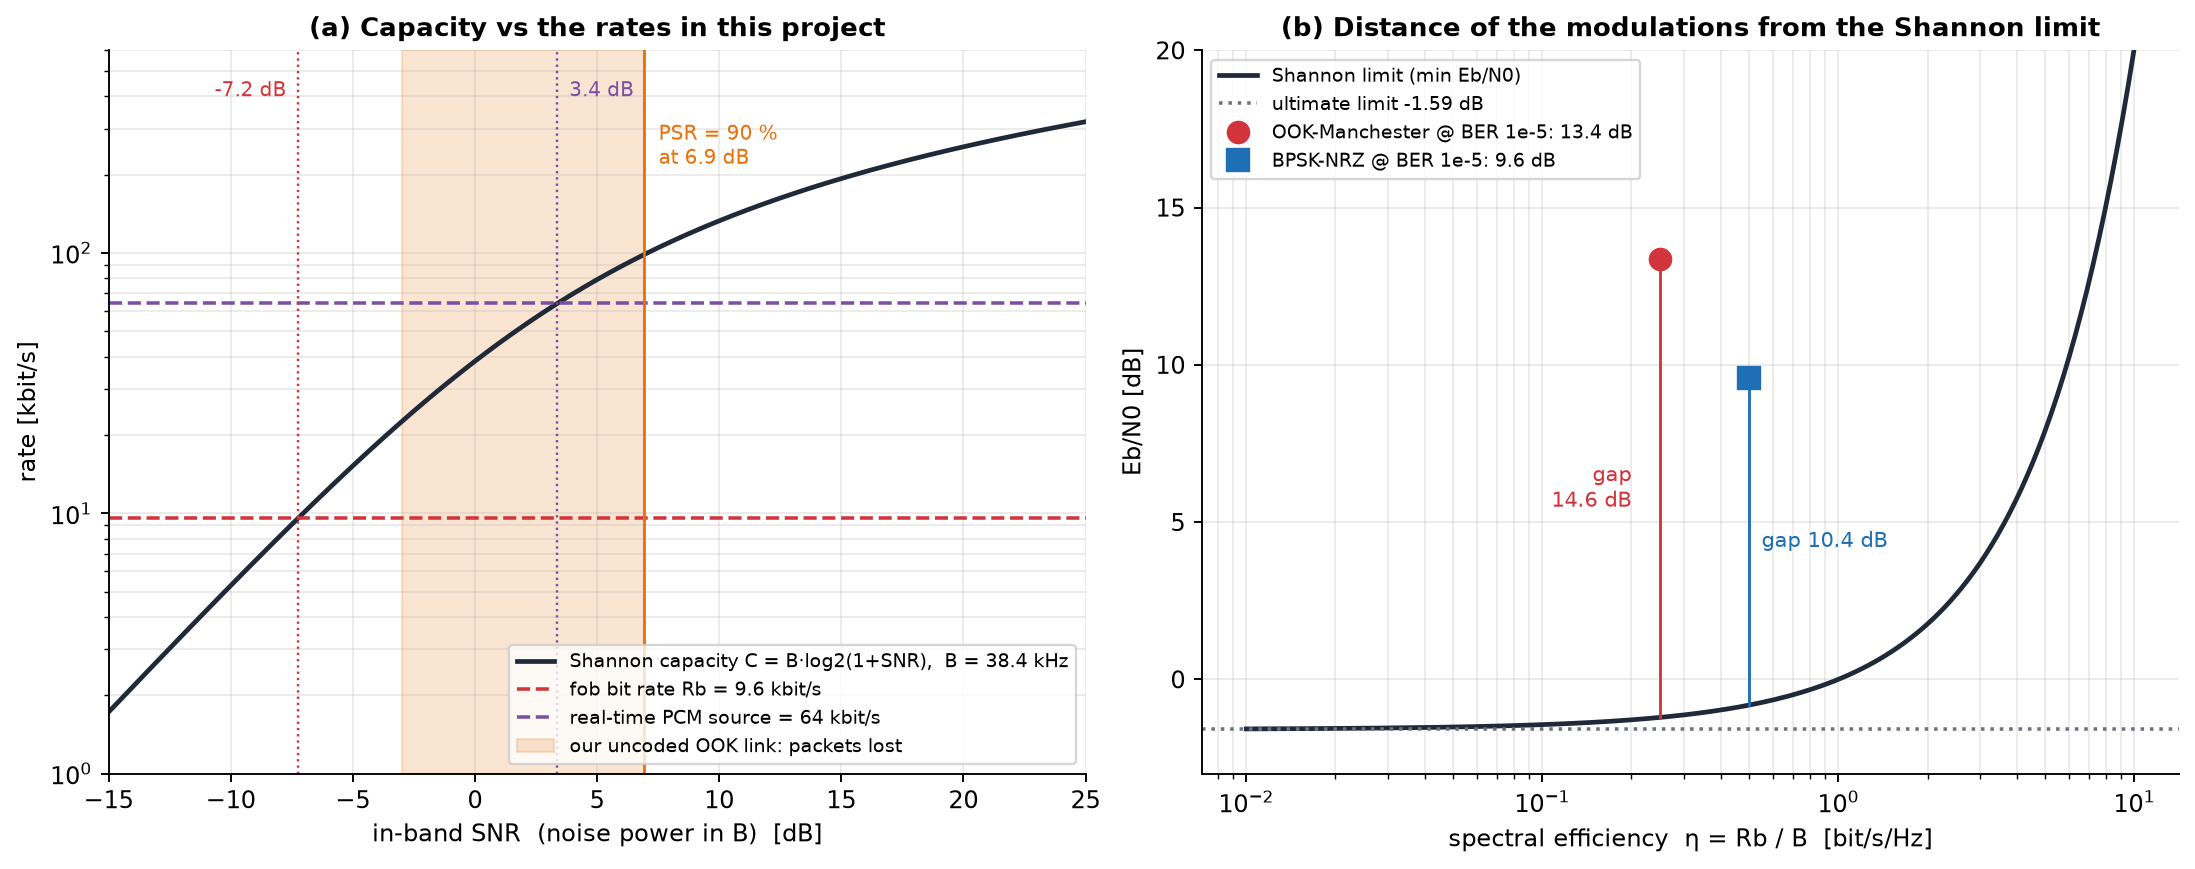
\includegraphics[width=\linewidth]{16_shannon.png}
\caption{(a) Capacity of the $B=38.4$~kHz channel against the fob bit rate and the real-time PCM rate. (b) $\EbNo$ needed for BER $=10^{-5}$ by our two modulations compared with the Shannon limit.}\end{figure}

\paragraph{Where is the channel the bottleneck?} There are three different answers, all visible in the figures.
\begin{enumerate}[leftmargin=1.4em,itemsep=2pt]
\item \textbf{Fundamental limit.} To carry $R_b=9.6$~kbit/s in $B=38.4$~kHz, any code and modulation needs an in-band SNR of at least @SH_SNR@~dB ($\EbNo\ge@SH_EB_OOK@$~dB). Below it the channel is the bottleneck for \emph{every} system.
\item \textbf{Practical limit of our link.} Our uncoded OOK link reaches 90\,\% packet success only at an in-band SNR of @PSR90_B@~dB, and the MSE leaves the quantization floor below @BSTAR@~dB. There the Shannon capacity is $@CAP90@$~kbit/s, about ten times the bit rate used: the channel is \emph{not} limiting for capacity reasons --- our modulation and the absence of error-correcting code are. The gap to the Shannon limit at BER $=10^{-5}$ is @GAP_OOK@~dB for OOK-Manchester ($\EbNo=@REQ_OOK@$~dB needed against @SH_EB_OOK@~dB) and @GAP_BPSK@~dB for BPSK-NRZ (@REQ_BPSK@~dB against @SH_EB_BPSK@~dB). Forward error correction, soft detection and coding of the MSBs could win back most of it.
\item \textbf{Rate bottleneck of the source.} Streaming the PCM audio in real time needs $F_s\cdot n=64$~kbit/s. Even an ideal coder needs an in-band SNR of @SH_SNR_SRC@~dB for this in 38.4~kHz, and our fob rate is 9.6~kbit/s: the 3200-bit clip needs @AIRTIME@~ms of airtime for 50~ms of audio, 6.7 times slower than real time. A fob therefore \emph{buffers and bursts} the payload, which is why we model a packet and not a stream.
\end{enumerate}
\textbf{Conclusion of the discussion.} At high SNR the \emph{source} (quantization, 8 bits) is the bottleneck and the MSE is flat. In a window of only about 5~dB around an in-band SNR of 7~dB the \emph{channel} takes over; the delivered MSE rises by almost five orders of magnitude (the raw MSE by nearly three), because one MSB error costs as much as 400 quantization noises. A designer should operate with a margin of several dB above that cliff (fading margin, Sec.~\ref{sec:range}) and, to approach the Shannon limit, spend bits on error protection of the MSBs instead of on more quantization levels.

%=====================================================================================
\section{Security layer: rolling code}\label{sec:security}
The hop code is a 32-bit block encrypted with a 528-round non-linear-feedback shift-register cipher modelled on KeeLoq (64-bit key shared by fob and car). The plaintext is
[4-bit command $|$ 12-bit discrimination (low bits of the serial number) $|$ 16-bit counter]. Every button press increments the counter. The car decrypts the hop code, checks the discrimination and command bits (a random hop code passes with probability $2^{-16}$) and compares the counter with the last accepted one (Fig.~\ref{fig:rcflow}).
This is a teaching simulation, not a secure implementation.

\begin{figure}[H]\centering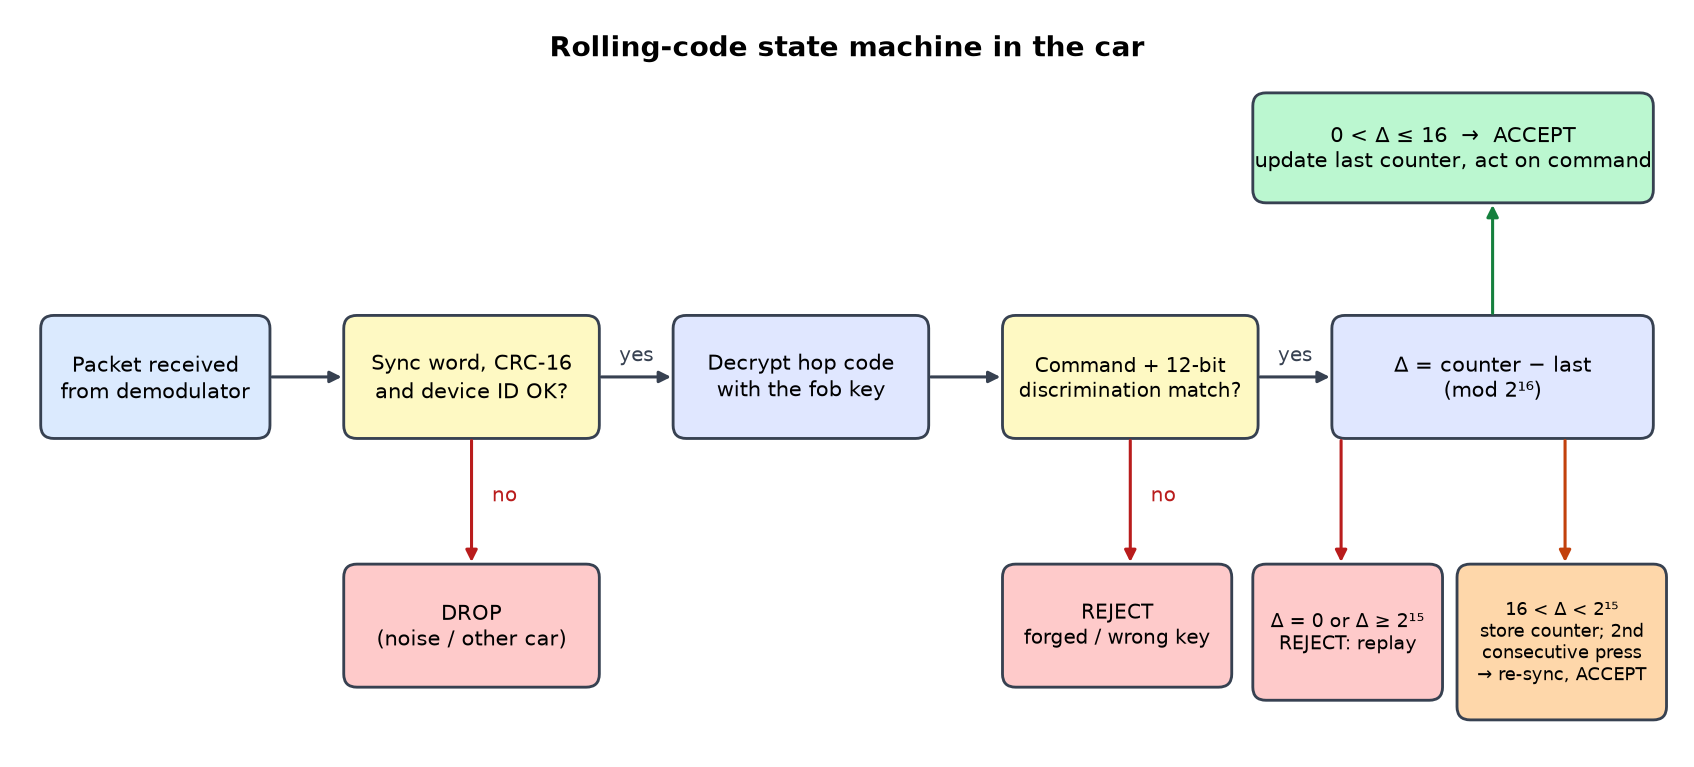
\includegraphics[width=\linewidth]{17_rolling_code_flow.png}
\caption{Receiver decision logic. $\Delta=$ counter $-$ last counter (mod $2^{16}$), look-ahead window 16.}\label{fig:rcflow}\end{figure}

We ran nine events through the \emph{full waveform chain} (modulation, channel, blind demodulation, frame parser, rolling-code check); Table~\ref{tab:events} and Fig.~\ref{fig:events} show the results.
In event 2 an attacker re-transmits a recording of event 1: the packet arrives perfectly (sync, CRC and ID all OK) and is nevertheless rejected because its counter was already used --- the security is in the counter, not in the radio link.

\begin{table}[H]\centering\scriptsize
\caption{Security demonstration (SNR 8 dB; event 6 at $-6$ dB).}\label{tab:events}
\begin{tabular}{@{}llp{4.6cm}rrlp{3.6cm}@{}}\toprule
\# & who & event & pkt ctr & car ctr & decision & reason\\\midrule
@TABLE_EVENTS@
\bottomrule\end{tabular}
\end{table}

\begin{figure}[H]\centering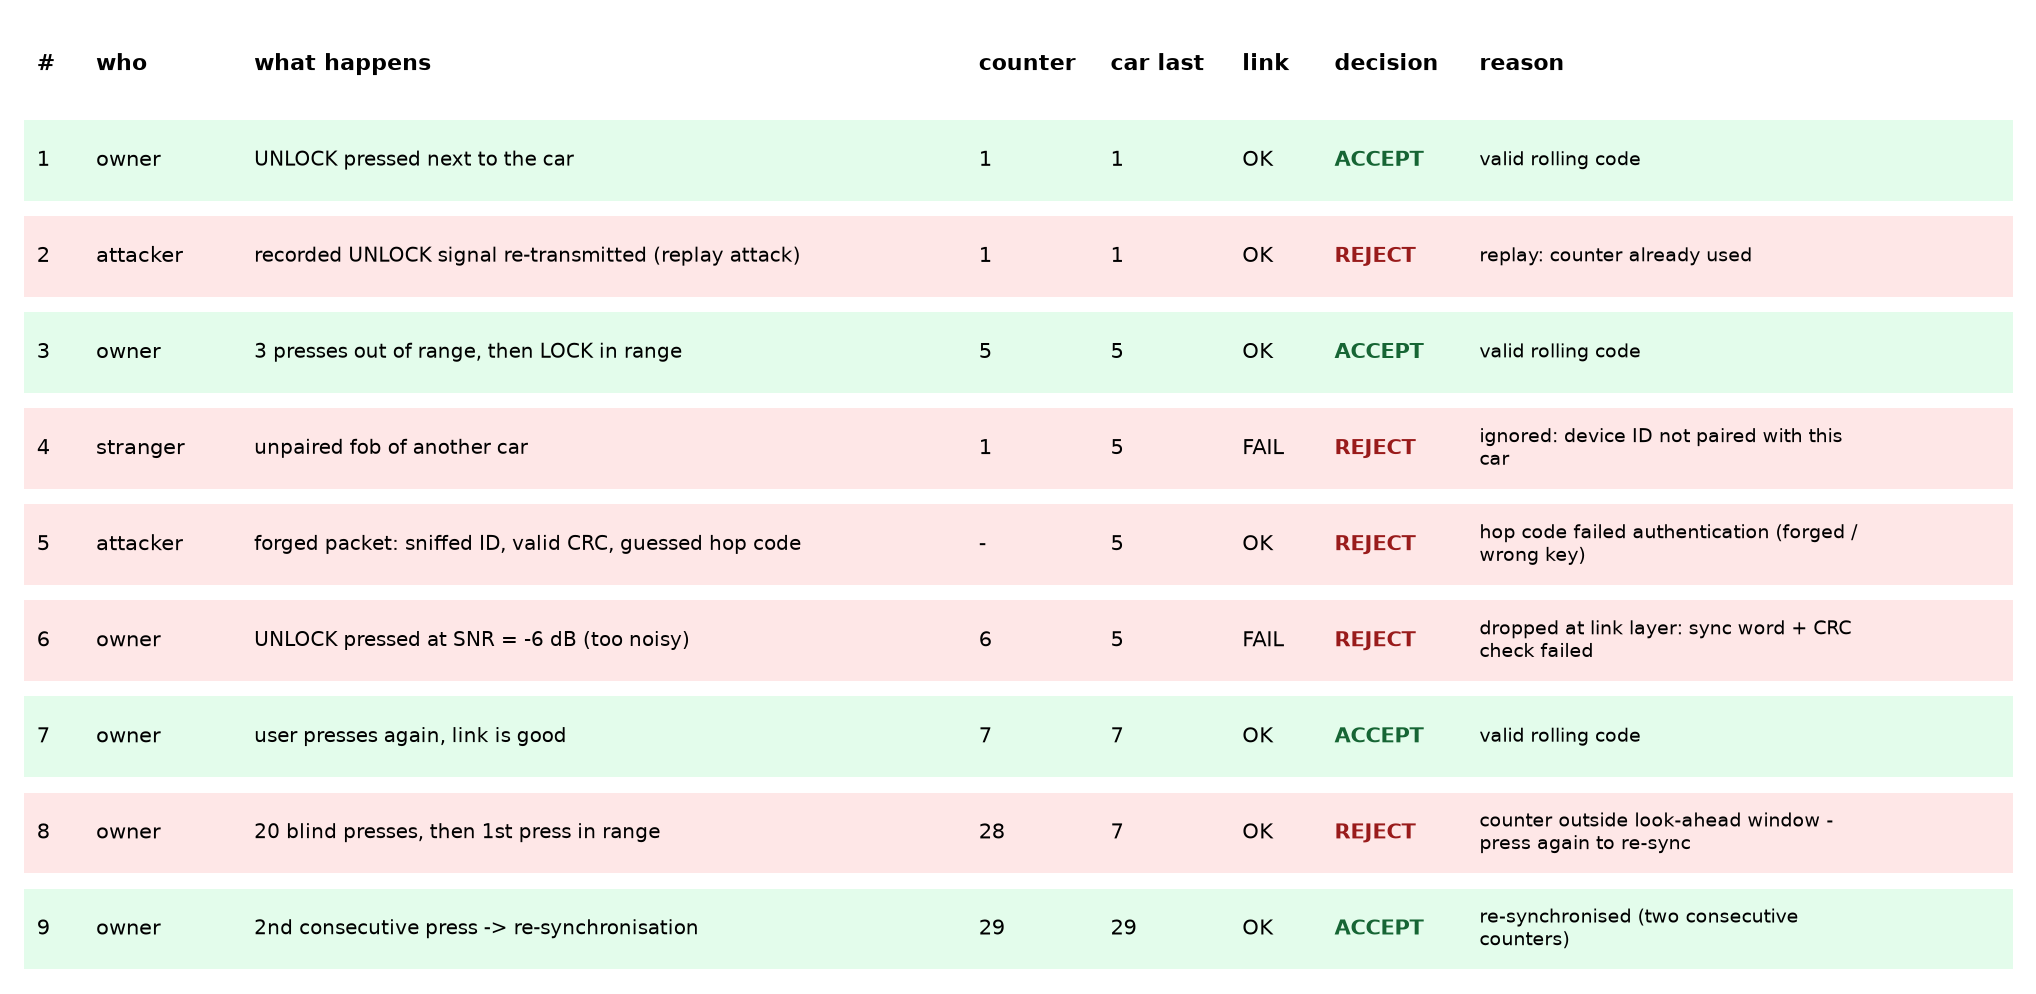
\includegraphics[width=\linewidth]{18_security_demo.png}
\caption{Security demonstration timeline.}\label{fig:events}\end{figure}

%=====================================================================================
\section{Range: from SNR to distance}\label{sec:range}
A log-distance link budget turns the SNR axis into metres: free-space loss at 1~m for 433.92~MHz (25.2~dB), path-loss exponent $n=3.5$ (obstructed), 15~dB extra body/car shadowing, fob EIRP $-15$~dBm, receiver noise floor @NF@~dBm
($kTB$ over 38.4~kHz plus 10~dB noise figure). Fading is modelled as flat and constant during one 346~ms packet (block fading): Rayleigh ($|h|^2$ exponential, no line of sight, like a parking garage) and Rician with $K=6$~dB (line of sight).
These link-budget numbers are \emph{illustrative assumptions}, not measurements.

\begin{figure}[H]\centering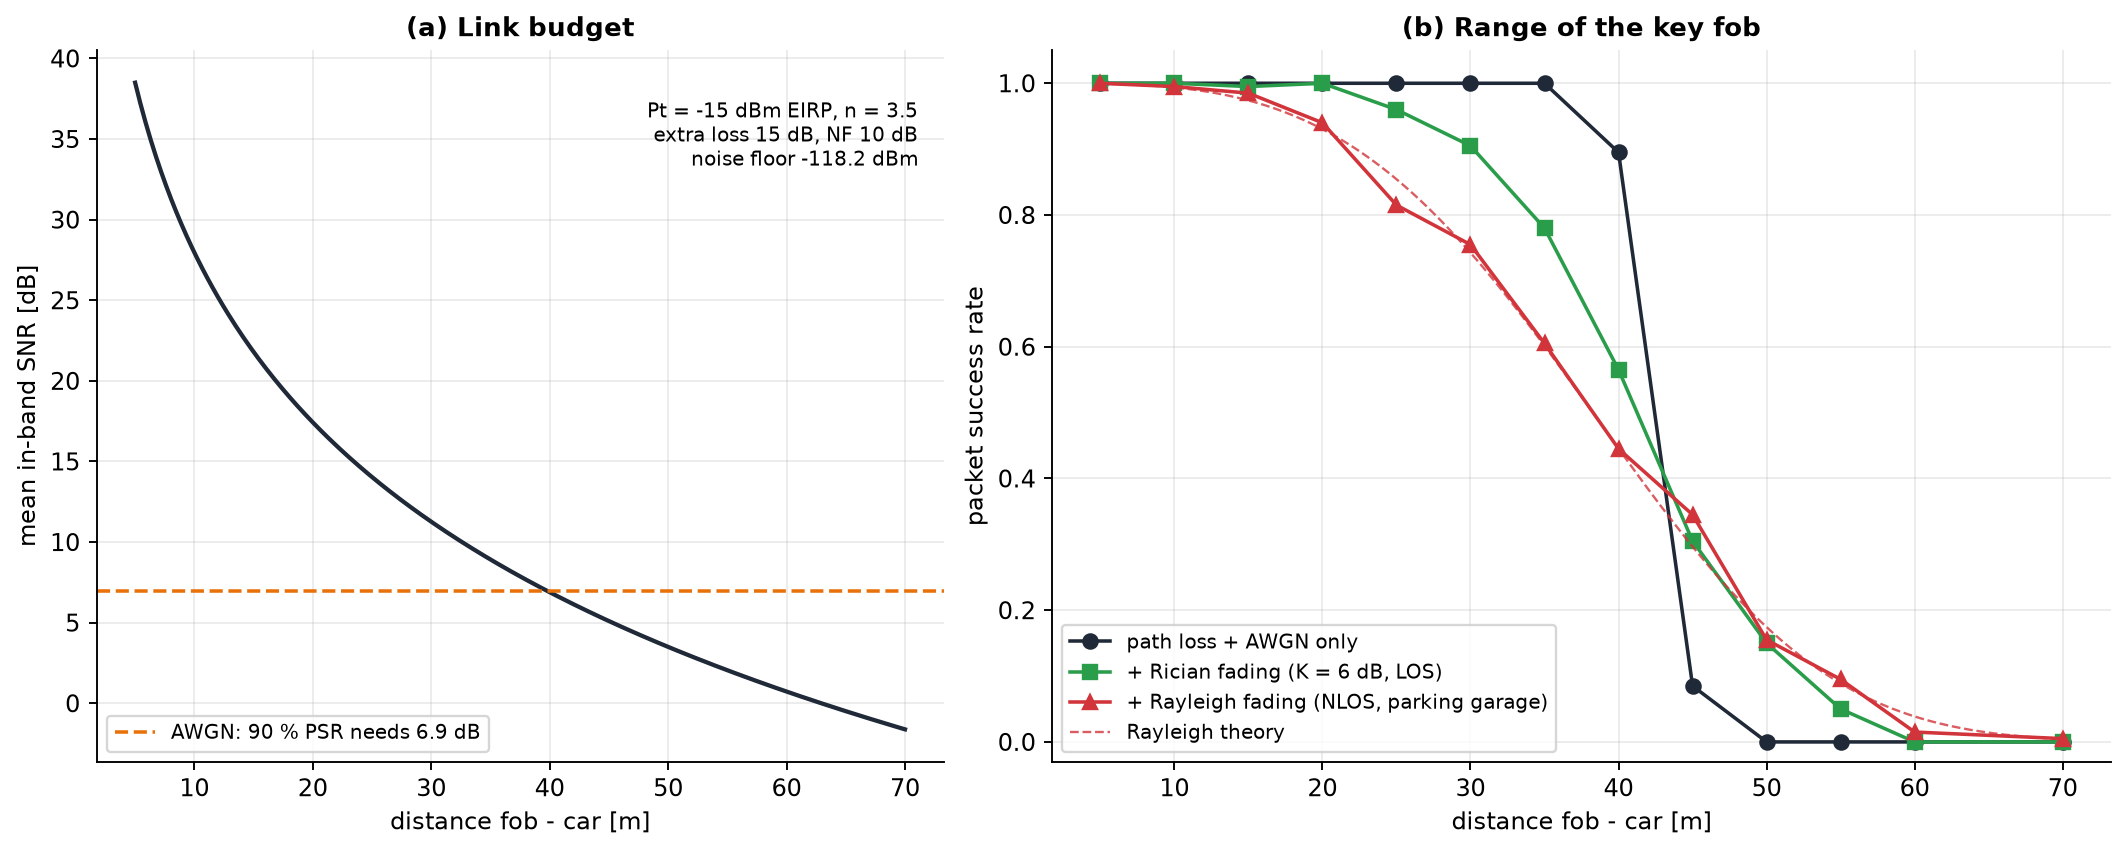
\includegraphics[width=\linewidth]{19_distance_range.png}
\caption{(a) Mean in-band SNR versus distance. (b) Packet success rate versus distance for three channels; the dashed line is the analytic Rayleigh average of the AWGN packet-success curve.}\end{figure}

\begin{table}[H]\centering\small
\caption{Packet success rate versus distance (@N_DIST@ packets per point).}
\begin{tabular}{@{}rrrrr@{}}\toprule
Distance [m] & SNR$_{\text{in-band}}$ [dB] & AWGN only & Rician $K$=6 dB & Rayleigh\\\midrule
@TABLE_DIST@
\bottomrule\end{tabular}
\end{table}

The 90\,\% range is about @R_AWGN@~m without fading, @R_RICIAN@~m with a line-of-sight component and @R_RAYLEIGH@~m with Rayleigh fading. Fading therefore costs almost half of the range: a deep fade of a few dB is enough to lose a 3320-bit packet whose CRC allows no error at all. This is why real fobs repeat the frame several times, and why the user simply presses the button again.

%=====================================================================================
\section{Verification, assumptions and limitations}
\paragraph{Verification.} (i) CRC-16 reproduces the standard check value \texttt{0x29B1}; (ii) KeeLoq-style encrypt/decrypt, PCM, quantizer and Manchester round trips, the clean-channel loop-back, rejection under heavy noise, replay/window/forgery rules are unit-tested (\texttt{tests/}, 12 tests, \texttt{python -m unittest discover -s tests});
(iii) the simulated BER matches theory for both OOK and BPSK (Fig.~\ref{fig:ber}) and the simulated MSE matches the analytic MSE($p$) (Fig.~\ref{fig:mse}); (iv) no undetected-error packet was observed. All results are reproducible with the seed in \texttt{Config}.

\paragraph{A pitfall we fixed.} Our first channel rotated the carrier phase with a Hilbert transform. With the scaled carrier ($f_c/R_b=4$) the OOK spectrum is not narrow compared with $f_c$, the transform leaked energy into the ``off'' chips and the BER was about 1.4--1.6 times too high.
The final channel uses the exact quadrature pair $\mathrm{Re}\{h\,(x_I+jx_Q)\}$, after which the simulation matches theory.

\paragraph{Assumptions and limitations.}
Scaled carrier (valid for error performance, see Sec.~2). Perfect sample-rate synchronisation between transmitter and receiver (no oscillator drift or frequency offset). No AGC, interference or multipath delay spread; flat block fading. KeeLoq-style cipher written from the published algorithm structure; it is not validated against official test vectors and is not meant to protect anything real.
Monte-Carlo confidence: a point with $k$ errors has a relative standard error of about $1/\sqrt{k}$; points with fewer than $\approx$30 errors (BER below $\approx2\times10^{-5}$) are indicative only. The link-budget parameters are assumptions.

\section{Conclusion}
We built and validated a complete, reproducible simulation of a key-fob link in which every block of the guideline chain is present and the physical-layer results agree with theory.
The reconstruction quality is flat at the 8-bit quantization limit of @SQNR@~dB until the channel SNR approaches about @BSTAR@~dB in-band, then collapses within a few dB; at the 90\,\% packet-success point the link is @GAP_SNR@~dB from the Shannon limit, so coding rather than capacity limits it. The rolling code makes recorded signals useless, and the link budget shows that fading, not noise alone, sets the useful range.

\section*{How to run and repository layout}
\begin{lstlisting}
pip install -r requirements.txt
python main.py            # full run (about 2-3 minutes) -> figures/, results/
python main.py --quick    # fast preview
python -m unittest discover -s tests -v
python report/build_report.py   # rebuilds report.pdf (needs LaTeX)
\end{lstlisting}
\begin{lstlisting}
main.py            entry point: runs the complete chain
functions/         config, source, quantizer, pcm, framing, rolling_code, line_coding,
                   modulation, channel, demodulation, receiver, reconstruction,
                   metrics, analysis, plots_*.py
figures/           all saved plots (01 ... 19)
results/           metrics.json and CSV tables of the sweeps
report.ipynb       the report as an executed notebook      report.pdf   this report
tests/             unit tests                              README.md
\end{lstlisting}

\begin{thebibliography}{9}
\bibitem{shannon} C.~E. Shannon, ``A mathematical theory of communication,'' \emph{Bell System Technical Journal}, 27, 1948.
\bibitem{proakis} J.~G. Proakis and M. Salehi, \emph{Digital Communications}, 5th ed., McGraw-Hill, 2008 (error probability of OOK/non-coherent and BPSK detection, Shannon limit).
\bibitem{keeloq} Microchip Technology, KeeLoq code-hopping encoder data sheets (HCS series) --- structure of the hop code and counter-window logic.
\end{thebibliography}
\end{document}
